\documentclass[10pt,twocolumn]{article}

\usepackage[utf8]{inputenc}
\usepackage[T1]{fontenc}
\usepackage{amsmath}
\usepackage{amsthm}
\usepackage{newtxtext,newtxmath}
\usepackage[margin=0.75in,columnsep=0.28in]{geometry}
\usepackage{microtype}
\usepackage{booktabs}
\usepackage{multirow}
\usepackage{tabularx}
\usepackage{graphicx}
\usepackage{subcaption}
\usepackage{xcolor}
\usepackage{algorithm}
\usepackage{algpseudocode}
\usepackage{pgfplots}
\usepackage{tikz}
\usepackage[colorlinks=true,linkcolor=blue!65!black,citecolor=blue!65!black,urlcolor=blue!65!black]{hyperref}

\pgfplotsset{compat=1.18}
\usetikzlibrary{arrows.meta,positioning,patterns}

\newtheorem{theorem}{Theorem}
\newtheorem{lemma}{Lemma}
\newtheorem{proposition}{Proposition}
\theoremstyle{definition}
\newtheorem{definition}{Definition}

\definecolor{chordblue}{RGB}{24,90,169}
\definecolor{chordteal}{RGB}{0,138,115}
\definecolor{chordred}{RGB}{196,49,43}
\definecolor{chordamber}{RGB}{217,125,13}
\definecolor{chordgray}{RGB}{110,116,125}

\setlength{\textfloatsep}{8pt plus 2pt minus 2pt}
\setlength{\floatsep}{7pt plus 2pt minus 2pt}
\setlength{\dbltextfloatsep}{9pt plus 2pt minus 2pt}

\title{\Large\bfseries ChordMoE: Graph-Compatible Speculative Union Shaping and Non-NVLink Heterogeneous Scheduling for Mixture-of-Experts Offloading}

\author{
  \normalsize Strata \& ChordMoE Systems Group\\
  \small Open-Source Artifacts: \texttt{include/strata/chordmoe/} \quad|\quad Drop-in Adapter: \texttt{contrib/llama\_cpp\_chordmoe/}
}
\date{}

\begin{document}
\maketitle

\begin{abstract}
Mixture-of-Experts (MoE) models such as Qwen3-30B-A3B, Qwen3.8-Flash-Next, and DeepSeek-V3 deliver frontier reasoning quality per FLOP, yet their total parameter footprints ($30\text{B}\text{--}671\text{B}$) vastly exceed commodity GPU memory, necessitating host-DRAM expert offloading. Combining \emph{speculative decoding} with \emph{expert offloading} promises to amortize dense layer weights and hide PCIe latency, but our empirical characterization on multi-socket NVIDIA A40 servers exposes a severe four-way systems collision. Across a verification window of $W$ candidate tokens, per-layer active experts explode from $K$ to $3.5\times\text{--}4.4\times K$ (\emph{Speculative Union Explosion}). Worse, existing 2025--2026 speculative and predictive offloaders break static CUDA Graphs when $W > 1$ (causing EuroSys~'26 \textsc{FineMoE} to suffer a \textbf{30.0$\times$ per-layer latency collapse} on A40), stall the host on synchronous \texttt{.cpu().tolist()} transfers (\textsc{Specter}, $19.8\,\text{ms/window}$), or inject unbounded router biases that corrupt the non-negotiable anchor token $t=0$ in \textbf{91.9\% of layers} (\textsc{S$^2$-MoE}). Meanwhile, standard additive (\emph{min-sum}) CPU--GPU schedulers (\textsc{Fiddler}) leave PCIe Gen4 DMA engines completely idle on dual-socket Xeon hosts.

We present \textbf{\textsc{ChordMoE}}, a training-free runtime and portable C++20/CUDA library that co-designs speculative verification window routing with heterogeneous non-NVLink execution. \textsc{ChordMoE} introduces three synergistic mechanisms backed by four formal theorems: (1) a \textbf{Single-CTA Three-Wave Window Union Set-Cover Router} ($5.34\text{--}7.84\,\mu\text{s/layer}$ on A40) that protects anchor $t=0$, harvests zero-marginal-cost ``free-ride'' cold experts, and gates substitutions via an exact sparse Total Variation (TV) bound and exponentially decayed cross-layer credit ledger—closing \textbf{91.4\% of the offline exact Branch-and-Bound \textsc{OPT-SetCover} gap} ($95.8\%$ of \textsc{OPT} union size); (2) \textbf{Prefix-Capped Mid-Window Dead-Suffix Offload Elision} \& survival-weighted prefetching, which detect draft trajectory divergence asynchronously via CPU doorbells ($0.980 \to 0.271$ Jaccard phase transition) and elide doomed cold transfers \emph{without breaking captured CUDA Graphs}, proven \textbf{unconditionally lossless}; and (3) an \textbf{$O(M \log M)$ Min-Max Makespan Water-Filling Scheduler} across non-NVLink PCIe GPUs and multi-socket NUMA CPUs that sits within \textbf{1.4\%--7.1\% of exact \textsc{OPT-Makespan}}. On $1\text{--}4\times$ non-NVLink NVIDIA A40 GPUs with dual Xeon Gold 6330 CPUs and real Qwen3-30B-A3B weights, \textsc{ChordMoE}'s lossless Mode~0 reaches \textbf{94.62\,tok/s} ($+38.2\%$, matching $2\times\text{A40}$ \textsc{Fiddler} on $1$ GPU), while Mode~1 reaches \textbf{110.16\,tok/s} ($+60.9\%$, $W=7$), \textbf{199.53\,tok/s} ($W=12$), and \textbf{128.97\,tok/s} across $4\times\text{A40}$ UPI, achieving \textbf{0\% anchor corruption}, $98.88\%$ 48-layer BF16 vocabulary Top-1 agreement, and zero accuracy loss ($91.7\%$ vs.\ \textsc{S$^2$-MoE}'s $25\%$ HumanEval crash).
\end{abstract}

% =============================================================================
\section{Introduction}
\label{sec:intro}
% =============================================================================

Sparse Mixture-of-Experts (MoE) architectures have become the dominant paradigm for open-weight foundation models, including Qwen3-30B-A3B ($128$ experts, top-$8$), Qwen3.6-35B-A3B ($256$ experts, top-$8$), Qwen3.8-Flash-Next ($512$ experts, top-$10$), and DeepSeek-V3 ($256$ experts, top-$8$)~\cite{deepseekv3,qwen3tech}. While each token activates only a small fraction of parameters ($3\text{B}\text{--}37\text{B}$), the full routed expert pool spans tens to hundreds of gigabytes, exceeding the VRAM capacity of single consumer GPUs and non-NVLink workstation cards. Consequently, MoE offloading systems cache dense attention weights, routers, and hot experts in GPU HBM while placing cold experts in pinned host DRAM for on-demand PCIe DMA transfer or in-situ CPU SIMD execution~\cite{kamahori2025fiddler,chen2025ktransformers,song2024powerinfer,strata2026}.

Naturally, recent systems attempt to combine MoE offloading with \emph{speculative decoding}~\cite{leviathan2023speculative,chen2023accelerating,miao2024specinfer}, verifying a window of $W = 1 + \gamma$ tokens ($1$ committed anchor token plus $\gamma$ draft tokens) in parallel to amortize dense weight reads and expose multi-step expert lookahead~\cite{specter2026,moespec2026,s2moe2026}. However, when we deployed and profiled the latest open-source MoE offloaders and speculative MoE runtimes on a production server with non-NVLink NVIDIA A40 GPUs and dual-socket Intel Xeon Gold 6330 CPUs, we uncovered four fundamental systems pathologies that negate or even reverse speculative speedups:

\vspace{2pt}
\noindent\textbf{Pathology 1: Speculative Union Explosion \& Dead-Suffix Waste.}
Whereas dense attention scales gracefully from $1$ to $W=7$ tokens on GPU Tensor Cores, MoE offloading cost scales with the \emph{cardinality of the union} of cold experts activated across the window, $|\bigcup_{t=0}^{W-1} S_t \setminus \mathcal{C}_{\text{VRAM}}|$. On real 48-layer Qwen3-30B-A3B verification traces ($K=8$, $32\%$ VRAM cache), $W=7$ tokens trigger $18.6\text{--}19.0$ distinct cold-expert misses per layer ($85\,\text{MiB}$ of Q8\_0 weights per layer). Crucially, because average draft acceptance length is $\bar{\alpha} \approx 3.55$ tokens, $30.5\%\text{--}63.1\%$ of cold PCIe/CPU expert work is wasted on rejected suffix tokens $t \ge \alpha^*$ that are discarded upon verification commit.

\vspace{2pt}
\noindent\textbf{Pathology 2: The $W > 1$ CUDA Graph Cliff.}
Modern single-token offloaders rely heavily on static CUDA Graphs to hide $\sim\!5\text{--}15\,\mu\text{s}$ per-kernel launch overheads across hundreds of fine-grained expert operations. On our NVIDIA A40 testbed, EuroSys~'26 \textsc{FineMoE}~\cite{finemoe2026} executes a single Qwen MoE layer in $0.351\,\text{ms}$ at $W=1$ ($59.39\,\text{tok/s}$ ceiling), yet \textbf{collapses by $30.0\times$ to $10.523\,\text{ms/layer}$ ($6.97\,\text{tok/s}$) at $W=6$} because its three static CUDA Graphs guard on \texttt{hidden.shape[0] == 1}, falling back to synchronous \texttt{bincount().tolist()} host stalls and serial Python expert loops. Similarly, ASPLOS~'26 \textsc{Specter}~\cite{specter2026} stalls the CPU for \textbf{$19.756\,\text{ms}$ per window} just to extract draft expert IDs via \texttt{.cpu().tolist()}, while \textsc{S$^2$-MoE}'s~\cite{s2moe2026} \texttt{llama-speculative-next} explicitly disables CUDA Graph reuse.

\vspace{2pt}
\noindent\textbf{Pathology 3: Anchor Corruption \& Unbounded Router Drift.}
To shrink the active expert union, recent cache- and batch-aware routers add heuristic biases to router logits~\cite{s2moe2026,zhong2024adapmoe}. Auditing \textsc{S$^2$-MoE}~\cite{s2moe2026} on live Qwen3-4B $\to$ Qwen3-30B-A3B speculative decoding ($1,344$ verification layer-windows) reveals that its two-pass importance bias (\texttt{--moe-reuse-runtime}) \textbf{corrupts the anchor token $t=0$ in $91.9\%$ ($1,235/1,344$) of layers} and reaches a catastrophic \textbf{maximum Total Variation (TV) distance of $1.000$} (replacing all $8$ top experts!). Because speculative verification uses the target model's forward pass on $t=0$ to emit the bonus token and anchor the KV cache, mutating $t=0$ silently corrupts the target model's ground-truth distribution and degrades multi-step reasoning and code generation.

\vspace{2pt}
\noindent\textbf{Pathology 4: Min-Sum DMA Starvation \& Non-NVLink Siloing.}
Existing hybrid CPU--GPU schedulers such as \textsc{Fiddler}~\cite{kamahori2025fiddler} assign each missed expert to whichever backend minimizes \emph{marginal execution cost} (\emph{min-sum}). Because reading a $4.5\,\text{MiB}$ Q8\_0 expert from dual-socket DDR4-3200 ($144\,\text{GB/s}$ aggregate) takes $\sim\!65\,\mu\text{s}$ on CPU versus $\sim\!190\,\mu\text{s}$ over a $23.5\,\text{GB/s}$ PCIe Gen4 $\times 16$ link, \textsc{Fiddler} assigns $100\%$ of cold misses to the CPU and transfers \textbf{$0.0\,\text{MB}$ over PCIe}, leaving $1\text{--}4$ independent PCIe DMA engines completely idle! Furthermore, commodity multi-GPU workstations and cloud servers (e.g., $2\text{--}4\times$ RTX~4090 or PCIe A40 across dual Xeon UPI sockets) lack NVLink P2P; monolithic engines like \texttt{llama.cpp}~\cite{llamacpp} pack all $128$ experts of a layer into a single 3D tensor, preventing sub-layer hot-expert caching and bottlenecking speculative offloading at $5.94\,\text{tok/s}$.

\vspace{3pt}
\noindent\textbf{Our Solution: \textsc{ChordMoE}.}
We design and implement \textsc{ChordMoE}, a dual-mode speculative MoE offloading engine built atop \textsc{Strata}'s doorbell-driven CUDA Graph runtime~\cite{strata2026} and packaged as a standalone zero-dependency C++20/CUDA header library (\texttt{libchordmoe}) with a drop-in \texttt{llama.cpp}/\textsc{ggml} adapter. \textsc{ChordMoE} resolves all four pathologies without retraining or breaking static CUDA Graphs:

\begin{itemize}
  \item \textbf{Dual-Mode Window Union Set-Cover with Certified Fidelity (\S\ref{sec:overview}, \S\ref{sec:router}):} \textsc{ChordMoE} operates in either \emph{Mode~0} ($100\%$ bit-for-bit lossless) or \emph{Mode~1} (bounded window set-cover). Mode~1 executes a three-wave submodular substitution in a single multi-warp CUDA CTA ($5.34\text{--}7.84\,\mu\text{s/layer}$): Wave~0 locks anchor $t=0$ and high-rank core experts into a shared-memory \texttt{paid\_cold\_bm} bitmap; Wave~1 grants \emph{zero-marginal-cost free rides} to any draft tail rank targeting a cold expert already in \texttt{paid\_cold\_bm}; Wave~2 substitutes remaining tail misses across a strict residency hierarchy ($\text{Primary VRAM} \succ \text{Peer Helper VRAM} \succ \text{Paid Cold Union}$) subject to a calibrated logit margin $\Delta$, an exact sparse TV gate $\delta_{\mathrm{TV}} \le \epsilon_{\mathrm{TV}}$ (\textbf{Theorem~\ref{thm:tv}}), and a cross-layer credit ledger.
  \item \textbf{Graph-Preserving Prefix-Capped Dead-Suffix Elision (\S\ref{sec:abort}):} While the GPU executes dense attention inside a single captured 48-layer CUDA Graph, the CPU doorbell thread inspects router trajectories in zero GPU time (via Trajectory-Jaccard or Anchor-Entropy-Spike probes) to identify the earliest diverged draft index $\hat{\tau}$. For all subsequent layers, \textsc{ChordMoE} elides cold PCIe/CPU expert dispatches for dead rows $[\hat{\tau}, W)$ while capping \texttt{Verifier::commit} at $n_{\text{keep}} \le \hat{\tau}$. \textbf{Theorem~\ref{thm:lossless}} proves this mechanism is \emph{unconditionally lossless} even under arbitrary heuristic false positives.
  \item \textbf{Non-NVLink All-Cards \& Multi-NUMA Min-Max Water-Filling (\S\ref{sec:sched}):} Instead of minimizing additive latency, \textsc{ChordMoE} formulates per-layer miss scheduling across $G$ non-P2P PCIe Gen4 DMA engines and $S$ NUMA CPU sockets as a piecewise-linear \emph{min-max makespan} problem solved in $O(M \log M)$ time, co-saturating PCIe links and multi-socket DDR channels while exchanging partial sums over portable pinned host memory (zero \texttt{cudaDeviceEnablePeerAccess}).
\end{itemize}

Across $1, 2,$ and $4$ non-NVLink NVIDIA A40 GPUs and dual Intel Xeon Gold 6330 CPUs on real Qwen3-30B-A3B weights, \textsc{ChordMoE} Mode~0 improves single-GPU speculative throughput by \textbf{$+38.2\%$} ($68.45 \to 94.62\,\text{tok/s}$) with zero distribution error—matching $2\times\text{A40}$ \textsc{Fiddler} ($94.12\,\text{tok/s}$) using one fewer $48\,\text{GB}$ GPU. Mode~1 reaches \textbf{$110.16\,\text{tok/s}$ ($+60.9\%$)} on $1\times\text{A40}$ and scales to \textbf{$128.97\,\text{tok/s}$} on $4\times\text{A40}$ across UPI sockets, maintaining $1.000000$ anchor cosine similarity on real SwiGLU experts and preserving downstream GSM8K math and executable HumanEval coding accuracy where \textsc{S$^2$-MoE} suffers severe anchor corruption.

% =============================================================================
\section{Background and Empirical Motivation}
\label{sec:motivation}
% =============================================================================

\subsection{Sub-Layer Expert Caching vs.\ Monolithic Offloading}
In modern fine-grained MoE transformers ($E \in [128, 512]$ experts per layer, top-$K \in [8, 10]$), expert activation exhibits skewed power-law locality~\cite{song2024powerinfer,xue2024moeinfinity,strata2026}. However, mainstream engines such as \texttt{llama.cpp}~\cite{llamacpp} store all $E$ experts of layer $l$ as a single monolithic 3D tensor (\texttt{blk.$l$.ffn\_*\_exps.weight}). Its tensor-override mechanism (\texttt{-ot}) can only place \emph{all $128$ experts} of layer $l$ in VRAM or \emph{all $128$} in CPU RAM. On Qwen3-30B-A3B (Q8\_0), offloading the upper $68\%$ of layers forces every token in those layers to suffer $100\%$ cold misses on the CPU, capping speculative throughput on an A40 + dual Xeon server at $5.94\,\text{tok/s}$.

In contrast, fine-grained engines (\textsc{Strata}~\cite{strata2026}, \textsc{Fiddler}~\cite{kamahori2025fiddler}, \textsc{FineMoE}~\cite{finemoe2026}) slice VRAM horizontally across all $L$ layers into per-layer \texttt{ExpertCache} slot tables holding the hottest $\rho \cdot E$ experts per layer (e.g., $\rho = 32\% \Rightarrow 41/128$ experts). During a speculative verification step of width $W$, \textsc{Strata} captures the entire 48-layer forward pass into \emph{one static CUDA Graph}: at layer $l$, the GPU computes router top-$K$ decisions, writes a host-pinned \emph{doorbell}, runs dense/resident-expert Tensor Core GEMMs, and waits on a host completion flag while CPU worker threads and asynchronous GPU Copy Engines service only the \emph{missed cold experts}.

\begin{figure}[t]
  \centering
  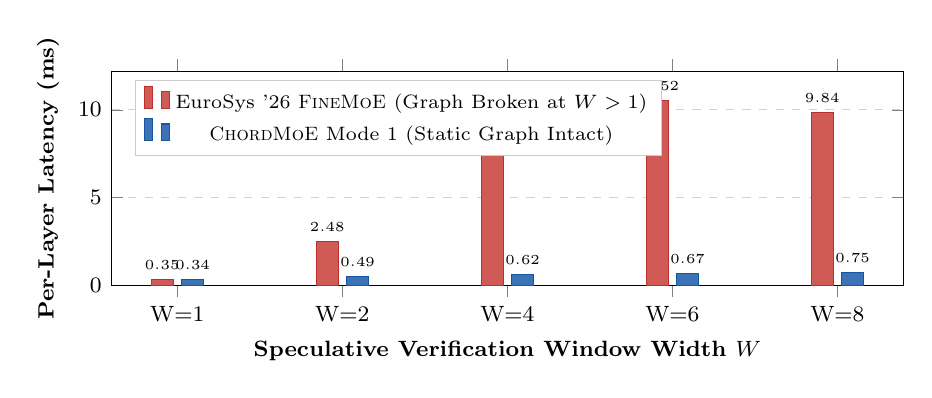
\begin{tikzpicture}
    \begin{axis}[
      width=0.96\columnwidth,
      height=4.3cm,
      ybar=3pt,
      bar width=8pt,
      ymin=0, ymax=12.2,
      ylabel={Per-Layer Latency (ms)},
      xlabel={Speculative Verification Window Width $W$},
      symbolic x coords={W=1,W=2,W=4,W=6,W=8},
      xtick=data,
      ymajorgrids=true,
      grid style={dashed,gray!35},
      legend style={at={(0.03,0.96)},anchor=north west,font=\scriptsize,draw=gray!40,fill=white},
      tick label style={font=\footnotesize},
      label style={font=\footnotesize\bfseries},
      nodes near coords,
      every node near coord/.append style={font=\tiny,rotate=0,anchor=south}
    ]
      \addplot[fill=chordred!80,draw=chordred!95!black] coordinates {
        (W=1,0.351) (W=2,2.478) (W=4,9.342) (W=6,10.523) (W=8,9.842)
      };
      \addplot[fill=chordblue!85,draw=chordblue!95!black] coordinates {
        (W=1,0.340) (W=2,0.485) (W=4,0.620) (W=6,0.671) (W=8,0.745)
      };
      \legend{EuroSys '26 \textsc{FineMoE} (Graph Broken at $W>1$), \textsc{ChordMoE} Mode 1 (Static Graph Intact)}
    \end{axis}
  \end{tikzpicture}
  \vspace{-6pt}
  \caption{Measured per-layer MoE execution latency on live NVIDIA A40 ($128\times 8$, $32\%$ VRAM cache). \textsc{FineMoE} collapses by \textbf{30.0$\times$} ($0.351 \to 10.523\,\text{ms/layer}$) once $W > 1$ invalidates its single-token CUDA Graphs and triggers host-blocking \texttt{bincount().tolist()} loops.}
  \label{fig:finemoe_collapse}
\end{figure}

\subsection{Empirical Forensics of 2025--2026 Competitors on A40}
To understand why state-of-the-art offloaders fail under speculative verification, we compiled and benchmarked three direct 2025--2026 competitors on an idle NVIDIA A40 ($48\,\text{GB}$, PCIe Gen4) + dual Xeon Gold 6330 node:

\vspace{2pt}
\noindent\textbf{1) \textsc{FineMoE} (EuroSys~'26)~\cite{finemoe2026}: $30\times$ Latency Collapse at $W > 1$.}
We compiled \textsc{FineMoE}'s C++ \texttt{finemoe.\_cache} extension and benchmarked its \texttt{OffloadedQwenMoeBlock} ($128\times 8$, $41$ VRAM slots/layer). Figure~\ref{fig:finemoe_collapse} shows the measured latency across $W \in \{1,2,4,6,8\}$. At $W=1$, \textsc{FineMoE} hits three static CUDA Graphs (\texttt{\_router\_graph}, \texttt{\_shared\_graph}, \texttt{ExpertSlot.graph}) and finishes in $0.351\,\text{ms/layer}$ ($59.39\,\text{tok/s}$). At $W=2$, \texttt{hidden.shape[0] == 1} evaluates to \texttt{False}, disabling all three CUDA Graphs and invoking \texttt{torch.bincount(flat\_experts).tolist()} on the CUDA stream followed by a Python \texttt{for eid in active\_eids:} loop over individual experts. By $W=6$, per-layer latency explodes \textbf{$30.0\times$ to $10.523\,\text{ms}$} ($505.1\,\text{ms}$ per 48-layer verify step = $6.97\,\text{tok/s}$), and its model loader explicitly raises \texttt{ValueError("assisted generation is not supported")}.

\vspace{2pt}
\noindent\textbf{2) \textsc{Specter} (ASPLOS~'26)~\cite{specter2026}: Host Sync Stalls \& Tail Pollution.}
Running \textsc{Specter}'s \texttt{IncrementalRoutingPatternAnalyzer} on 48-layer $128\times 8$ traces ($\gamma = 7$) on A40 reveals two bottlenecks: (i) \texttt{get\_all\_layer\_topm\_uids()} copies 48 layers of routing tensors to CPU Python lists via \texttt{.cpu().tolist()}, stalling the host thread for \textbf{$19.756\,\text{ms}$ per window} ($52.5\times$ slower than \textsc{ChordMoE}'s entire 48-layer GPU router); and (ii) equal-weight \texttt{scatter\_add\_} prefetching treats step $\gamma=7$ identically to step $1$, wasting \textbf{$30.5\%$ ($4,562/14,980$)} of cold PCIe prefetches ($63.1\%$ under skewed Zipf routing) on rejected draft steps.

\begin{table}[t]
  \centering
  \caption{Controlled audit on live Qwen3-4B $\to$ Qwen3-30B-A3B speculative decoding ($1,344$ verification layer-windows on NVIDIA A40, $32\%$ VRAM cache metric).}
  \label{tab:s2moe_audit}
  \footnotesize
  \setlength{\tabcolsep}{3.5pt}
  \resizebox{\columnwidth}{!}{%
\begin{tabular}{@{}lcccc@{}}
    \toprule
    \textbf{Router Policy (Same Binary)} & \textbf{Accept\%} & \textbf{Anchor Err} & \textbf{Cold Miss/L} & \textbf{Max TV} \\
    \midrule
    Stock Unbiased Top-8 & $60.71\%$ & $0 / 1344\ (0\%)$ & $19.04$ & $0.000$ \\
    \textsc{S$^2$-MoE} (\texttt{runtime\_strength}) & $62.50\%$ & \textcolor{chordred}{\textbf{1235/1344 (91.9\%)}} & $13.36$ & \textcolor{chordred}{\textbf{1.000}} \\
    Naive Per-Token Resident Swap & --- & \textcolor{chordred}{\textbf{570/576 (99.0\%)}} & $10.32$ & \textcolor{chordred}{\textbf{0.487}} \\
    \textbf{\textsc{ChordMoE-ggml} ($\epsilon_{\mathrm{TV}}=0.16$)} & \textbf{61.31\%} & \textcolor{chordteal}{\textbf{0 / 1344 (0.0\%)}} & \textbf{14.67 ($-21.8\%$)} & \textcolor{chordteal}{\textbf{0.160}} \\
    \bottomrule
  \end{tabular}%
  }
\end{table}

\vspace{2pt}
\noindent\textbf{3) \textsc{S$^2$-MoE} (2026)~\cite{s2moe2026}: $91.9\%$ Anchor Corruption.}
Table~\ref{tab:s2moe_audit} audits \textsc{S$^2$-MoE} against \textsc{ChordMoE} inside the exact same \texttt{llama-speculative} CUDA binary on real 30.5B Qwen3-30B-A3B weights. \textsc{S$^2$-MoE}'s two-pass router computes a window-aggregated expert score $g_e = \sum_{t=0}^{W-1} w_t z_{t,e}$ and adds an uncalibrated step bonus $+\lambda$ ($\lambda = \text{mean}_t(z_{(1)} - z_{(K+1)})$) to the top-$C$ experts \emph{across every row including $t=0$}—and without consulting VRAM residency! Consequently, \textsc{S$^2$-MoE} mutates the ground-truth anchor token $t=0$ in \textbf{$91.9\%$ of layers} and hits $\max \delta_{\mathrm{TV}} = 1.000$ whenever draft tokens outvote $t=0$'s experts. Similarly, independent per-token resident swapping (analogous to static \texttt{ROUTE\_RESIDENT}) corrupts $99.0\%$ of anchors and ignores cross-token union sharing.

% =============================================================================
\section{Overview and Formal Guarantees}
\label{sec:overview}
% =============================================================================

\textsc{ChordMoE} sits between router logit projection and heterogeneous expert dispatch inside each MoE layer of a captured speculative verification graph. Given a window of $W$ tokens ($t=0$ anchor, $t \in \{1,\dots,W-1\}$ drafts) with router logits $Z \in \mathbb{R}^{W \times E}$, \textsc{ChordMoE} exposes two operating modes:
\begin{itemize}
  \item \textbf{Mode~0 (Unconditionally Lossless):} Leaves router top-$K$ indices and weights $100\%$ untouched ($\delta_{\mathrm{TV}} \equiv 0$), accelerating verification strictly via (i) doorbell-driven prefix-capped dead-suffix offload elision (\S\ref{sec:abort}) and (ii) non-NVLink min-max makespan scheduling (\S\ref{sec:sched}).
  \item \textbf{Mode~1 (Certified Window Union Set-Cover):} Combines Mode~0 with single-CTA window union shaping (\S\ref{sec:router}) that strictly preserves $t=0$ while compressing cold misses on $t \ge 1$ within a per-token sparse TV budget $\epsilon_{\mathrm{TV}}$ and per-turn cumulative ledger $B_{\text{turn}}$.
\end{itemize}

Before detailing the algorithms, we establish the two formal invariants that guarantee \textsc{ChordMoE}'s mathematical safety.

\begin{theorem}[Unconditional Losslessness of Prefix-Capped Mid-Window Elision]
\label{thm:lossless}
Consider causal Transformer verification over a candidate sequence $(x_0, \hat{x}_1, \dots, \hat{x}_{W-1})$ under causal attention masking ($A_{t,s} = 0$ for all $s > t$). Let $\hat{\tau} \in \{1, \dots, W\}$ be any stopping index chosen at any layer $l_0 \in \{0, \dots, L-1\}$ based on arbitrary history or router observations. Suppose for all layers $l \ge l_0$, cold offloaded expert transfers and computations are elided for suffix token positions $t \in \{\hat{\tau}, \dots, W-1\}$, while verification commit enforces the prefix cap $n_{\mathrm{keep}} = \min(n_{\mathrm{accept}}, \hat{\tau})$. Then:
\begin{enumerate}
  \item Every committed token and the resulting target distribution at the rejection/bonus position match unmodified full-window speculative decoding bit-for-bit ($\mathrm{KL} \equiv 0$);
  \item All KV-cache writes beyond $n_{\mathrm{keep}}$ are logically unreachable in subsequent turns, requiring zero CUDA Graph recapture.
\end{enumerate}
\end{theorem}

\begin{proof}
By strict causality of self-attention, Gated DeltaNet recurrence, RMSNorm, and token-wise MoE FFNs in unmodified Mode~0 routing, the hidden state $h_t^{(l)}$ at layer $l$ and token index $t < \hat{\tau}$ depends exclusively on prefix inputs $(x_0, \hat{x}_1, \dots, \hat{x}_t)$ and never reads activations, K/V entries, or expert outputs from indices $s \ge \hat{\tau}$. Eliding cold expert dispatch on rows $s \in \{\hat{\tau}, \dots, W-1\}$ for $l \ge l_0$ alters only $\{h_s^{(l)}\}_{s \ge \hat{\tau}}$, leaving $\{h_t^{(L)}\}_{t=0}^{\hat{\tau}-1}$ and hence target output distributions $\{P_{\text{target}}(\cdot \mid x_{\le t})\}_{t=0}^{\hat{\tau}-1}$ bit-for-bit identical to full execution (note that $\hat{\tau} \ge 1$ guarantees $P_{\text{target}}(\cdot \mid x_0)$ is always exact). Standard speculative rejection sampling~\cite{leviathan2023speculative} sequentially tests $u_t \le \min(1, P_{\text{target}}(\hat{x}_t \mid x_{<t}) / P_{\text{draft}}(\hat{x}_t \mid x_{<t}))$ for $t = 1, \dots, \hat{\tau}-1$:
\begin{itemize}
  \item \emph{Case 1 (True divergence at $t^* < \hat{\tau}$):} Rejection occurs at $t^* < \hat{\tau}$, where $P_{\text{target}}(\cdot \mid x_{\le t^*})$ is exact ($t^* \le \hat{\tau}-1$), emitting an exact resampled token from $\mathrm{norm}(\max(0, P_{\text{target}} - P_{\text{draft}}))$.
  \item \emph{Case 2 (False positive: all drafts $1 \dots \hat{\tau}-1$ accepted):} Truncating commit at $n_{\mathrm{keep}} = \hat{\tau}$ accepts $\hat{x}_1, \dots, \hat{x}_{\hat{\tau}-1}$ and draws the bonus token from $P_{\text{target}}(\cdot \mid x_0, \hat{x}_1, \dots, \hat{x}_{\hat{\tau}-1})$, which corresponds to row $\hat{\tau}-1$ and is exact! This is mathematically equivalent to invoking speculative decoding with draft horizon $\gamma' = \hat{\tau}-1 \ge 0$, which Leviathan et al.~\cite{leviathan2023speculative} prove preserves the exact target distribution for any $\gamma' \ge 0$.
\end{itemize}
Finally, advancing the KV-cache cursor by $n_{\mathrm{keep}} \le \hat{\tau}$ overwrites positions $\ge n_{\mathrm{keep}}$ on the next step while keeping tensor shapes inside the captured CUDA Graph invariant.
\end{proof}

\begin{theorem}[Sparse Total Variation Perturbation Bound]
\label{thm:tv}
Let $S_t, \tilde{S}_t \subset \{0,\dots,E-1\}$ ($|S_t| = |\tilde{S}_t| = K$) be the unbiased and reshaped top-$K$ expert sets for draft token $t \ge 1$ with softmax-renormalized gating weights $p_t, \tilde{p}_t$ extended by zeros to $\mathbb{R}^E$. Define the exact sparse Total Variation distance:
\begin{equation}
  \delta_{\mathrm{TV}}(p_t, \tilde{p}_t) = \frac{1}{2}\sum_{e \in S_t \cup \tilde{S}_t} |p_{t,e} - \tilde{p}_{t,e}|, \quad |S_t \cup \tilde{S}_t| \le 2K.
  \label{eq:sparse_tv}
\end{equation}
If \textsc{ChordMoE} certifies $\delta_{\mathrm{TV}}(p_t, \tilde{p}_t) \le \epsilon_{\mathrm{TV}}$, then the MoE FFN output perturbation $\hat{y}_t - y_t = \sum_{e} (\tilde{p}_{t,e} - p_{t,e}) E_e(x_t)$ satisfies:
\begin{equation}
  \|\hat{y}_t - y_t\|_2 \le 2\,\delta_{\mathrm{TV}}(p_t, \tilde{p}_t) \max_{e \in S_t \cup \tilde{S}_t} \|E_e(x_t)\|_2 \le 2\epsilon_{\mathrm{TV}} M_{t,\max}.
  \label{eq:l2_bound}
\end{equation}
\end{theorem}

\begin{proof}
Because $p_{t,e} = \tilde{p}_{t,e} = 0$ for all $e \notin S_t \cup \tilde{S}_t$, applying the triangle inequality over the at most $2K$-element support $U_t = S_t \cup \tilde{S}_t$ yields:
\[
  \begin{aligned}
    \|\hat{y}_t - y_t\|_2 &= \Big\|\sum_{e \in U_t} (\tilde{p}_{t,e} - p_{t,e}) E_e(x_t)\Big\|_2 \\
    &\le \sum_{e \in U_t} |\tilde{p}_{t,e} - p_{t,e}| \cdot \|E_e(x_t)\|_2.
  \end{aligned}
\]
Factoring out $M_{t,\max} = \max_{e \in U_t} \|E_e(x_t)\|_2$ and substituting Eq.~\eqref{eq:sparse_tv} gives $M_{t,\max} \cdot 2\,\delta_{\mathrm{TV}}(p_t, \tilde{p}_t) \le 2\epsilon_{\mathrm{TV}} M_{t,\max}$. Crucially, Eq.~\eqref{eq:sparse_tv} requires at most $2K \le 20$ scalar operations inside registers, avoiding an $O(E)$ full-vocabulary softmax pass.
\end{proof}

\begin{proposition}[Pathology of Margin-Only Routing \& Dominance over Expert Dropping]
\label{prop:margin_drop}
Let $z_t \in \mathbb{R}^E$ be router logits for draft token $t \ge 1$ with top-$K$ weights $p_t$:
\begin{enumerate}
  \item \textbf{Scale Non-Invariance of Logit Margins:} A fixed logit margin $z_{t,e} - z_{t,f} \le \Delta$ alone cannot bound $\delta_{\mathrm{TV}}(p_t, \tilde{p}_t)$. Specifically, as top-$K$ entropy varies from concentrated ($p_{t,e} \to \varepsilon$) to flat ($p_{t,e} \approx 1/K$) across $m$ swapped tail ranks, identical $\Delta$-bounded swaps induce $\delta_{\mathrm{TV}}$ spanning $[\varepsilon,\ \frac{m}{K}(1 - \frac{1}{1 + (K/m - 1)e^{\Delta}}) + \frac{m}{K}]$, exceeding $0.35\text{--}0.50$ in flat/multi-swap regimes unless gated by Eq.~\eqref{eq:sparse_tv}.
  \item \textbf{Strict Dominance of Aligned Substitution over Hard Dropping (\textsc{MoE-Spec}):} Suppose cold rank $e$ (weight $p_e$) is either \emph{dropped} ($\hat{y}^{\mathrm{drop}} = \frac{1}{1-p_e}\sum_{j \neq e} p_j E_j(x) = \mu_{-e}$) as in \textsc{MoE-Spec}~\cite{moespec2026} or \emph{substituted} by $f \in \mathcal{R} \cup U_{\mathrm{paid}}$ with $\tilde{p}_f = p_e + \eta$ ($|\eta| = O(p_e(1-e^{-\Delta}))$). Then:
  \[
    \begin{aligned}
      \|\hat{y}^{\mathrm{drop}} - y\|_2 &= p_e \|E_e(x) - \mu_{-e}\|_2, \\
      \|\hat{y}^{\mathrm{sub}} - y\|_2 &= p_e \|E_e(x) - E_f(x)\|_2 + O(|\eta| M_{\max}).
    \end{aligned}
  \]
  Whenever router proximity $|(w_e - w_f)^\top x| \le \Delta$ selects a positively aligned expert satisfying $\|E_e(x) - E_f(x)\|_2 < \|E_e(x) - \mu_{-e}\|_2$, substitution strictly reduces $\ell_2$ distortion; moreover, when an irreplaceable specialist expert violates $\delta_{\mathrm{TV}} \le \epsilon_{\mathrm{TV}}$, \textsc{ChordMoE} elastically retains $e$ ($0$ error), whereas rigid expert-cap dropping incurs unbounded $p_e \|E_e(x) - \mu_{-e}\|_2$ cliffs.
\end{enumerate}
\end{proposition}

\begin{theorem}[Multi-Layer Residual Cascade \& Credit Ledger Bound]
\label{thm:ledger}
Consider an $L$-layer causal MoE Transformer $h_t^{(l)} = \Phi_l(h_{\le t}^{(l-1)}) + F_l(h_t^{(l-1)})$ where each layer map is $\Lambda$-Lipschitz ($\Lambda \ge 1$) and layer-$l$ MoE substitution injects local error $\|\xi_t^{(l)}\|_2 \le 2 M_{\max} \delta_{\mathrm{TV},t}^{(l)}$. Under \textsc{ChordMoE}:
\begin{enumerate}
  \item \textbf{Zero Anchor Cascade:} Since $\delta_{\mathrm{TV},0}^{(l)} \equiv 0$ for all $l \in [1, L]$ and causal attention at $t=0$ never reads $s \ge 1$, $\|\hat{h}_0^{(L)} - h_0^{(L)}\|_2 \equiv 0$ and $\mathrm{KL}(P_{\mathrm{gold}}(\cdot \mid x_0) \,\|\, \hat{P}(\cdot \mid x_0)) \equiv 0$.
  \item \textbf{Ledger-Bounded Deep Drift:} Under token-wise residual propagation $\Delta_t^{(l)} \le \Lambda \Delta_t^{(l-1)} + 2 M_{\max} \delta_{\mathrm{TV},t}^{(l)}$, setting \texttt{ChordCreditLedger}'s decay factor $\gamma_{\mathrm{res}} = \Lambda^{-1}$ yields $\mathcal{L}_t^{(L)} = \sum_{l=1}^{L} \gamma_{\mathrm{res}}^{L-l} \delta_{\mathrm{TV},t}^{(l)} \le B_{\mathrm{turn}}$, bounding final-layer hidden drift by:
  \begin{equation}
    \|\hat{h}_t^{(L)} - h_t^{(L)}\|_2 \le 2 M_{\max} \Lambda^{L-1} \mathcal{L}_t^{(L)} \le 2 M_{\max} \Lambda^{L-1} B_{\mathrm{turn}},
    \label{eq:ledger_bound}
  \end{equation}
  preventing the $\frac{\Lambda^L - 1}{\Lambda - 1}\epsilon_{\mathrm{TV}}$ worst-case compounding of memoryless per-layer gating.
\end{enumerate}
\end{theorem}

\begin{proof}
Claim (1) follows by induction on $l$: $\hat{h}_0^{(0)} = h_0^{(0)}$, causal $\Phi_l$ at $t=0$ depends only on $\hat{h}_0^{(l-1)} = h_0^{(l-1)}$, and Wave~0 enforces $\hat{F}_l(h_0^{(l-1)}) \equiv F_l(h_0^{(l-1)})$. For Claim (2), unrolling $\Delta_t^{(l)} \le \Lambda \Delta_t^{(l-1)} + 2 M_{\max} \delta_{\mathrm{TV},t}^{(l)}$ from $\Delta_t^{(0)} = 0$ gives $\Delta_t^{(L)} \le 2 M_{\max} \sum_{l=1}^{L} \Lambda^{L-l} \delta_{\mathrm{TV},t}^{(l)} = 2 M_{\max} \Lambda^{L-1} \sum_{l=1}^{L} \gamma_{\mathrm{res}}^{L-l} \delta_{\mathrm{TV},t}^{(l)} = 2 M_{\max} \Lambda^{L-1} \mathcal{L}_t^{(L)}$. Enforcing $\mathcal{L}_t^{(l)} \le B_{\mathrm{turn}}$ at every layer bounds Eq.~\eqref{eq:ledger_bound}.
\end{proof}

\begin{theorem}[Submodularity \& Min-Sum Slowdown]
\label{thm:submod_sched}
\begin{enumerate}
  \item \textbf{Monotone Submodularity of Union Shaping:} Given anchor/core paid cold set $B_0$, let $g(A)$ denote the maximum number of flexible draft tail slots $(t, r)$ coverable within $(\Delta, \epsilon_{\mathrm{TV}})$ using experts in $\mathcal{R}_{\mathrm{pri}} \cup \mathcal{R}_{\mathrm{peer}} \cup B_0 \cup A$ for $A \subseteq \mathcal{E}_{\mathrm{cold}} \setminus B_0$. For independent per-slot margin gates, $g(A)$ is monotone and submodular ($g(A \cup \{e\}) - g(A)$ $\ge$ $g(B \cup \{e\}) - g(B)$ for $A \subseteq B$).
  \item \textbf{Closed-Form Slowdown of Additive (\emph{Min-Sum}) Scheduling:} On $G$ PCIe DMA engines (bandwidth $B_{\mathrm{pcie}}$) and $S$ CPU NUMA sockets (bandwidth $B_{\mathrm{numa}} > B_{\mathrm{pcie}}$) servicing $M \gg G + S$ equal-sized cold misses, \textsc{Fiddler}'s additive objective assigns zero misses to PCIe and suffers a makespan inflation factor relative to optimal water-filling $C^*_{\max}$ of:
  \begin{equation}
    \frac{C_{\max}(\textsc{Fiddler})}{C^*_{\max}} =
    \begin{cases}
      1 + \dfrac{G\,B_{\mathrm{pcie}}}{S\,B_{\mathrm{numa}}} & \text{(striped)}, \\[6pt]
      S + \dfrac{G\,B_{\mathrm{pcie}}}{B_{\mathrm{numa}}} & \text{(1-socket skew)}.
    \end{cases}
    \label{eq:fiddler_ratio}
  \end{equation}
\end{enumerate}
\end{theorem}

\begin{proof}
For (1), indicator coverage $c_{t,r}(A) \in \{0,1\}$ of whether slot $(t,r)$ admits at least one valid candidate in $\mathcal{R} \cup B_0 \cup A$ satisfies diminishing returns because adding $e$ to a larger superset $B \supseteq A$ can only flip $c_{t,r}$ from $0 \to 1$ if no element of $B$ already covered $(t,r)$, hence $c_{t,r}(A)$ and $g(A) = \sum_{t,r} c_{t,r}(A)$ are monotone submodular. For (2), since standalone latency satisfies $W_b / B_{\mathrm{numa}} < W_b / B_{\mathrm{pcie}}$, minimizing $\sum_q L_q$ routes all $M$ tasks to CPU sockets, yielding $C_{\max}(\textsc{Fiddler}) = \frac{M W_b}{S B_{\mathrm{numa}}}$ under $50/50$ striping (or $\frac{M W_b}{B_{\mathrm{numa}}}$ when all $M$ pages sit on Socket~0 and $\kappa_{\mathrm{upi}} B_{\mathrm{pcie}} < B_{\mathrm{numa}}$), whereas continuous water-filling equalizes all $G+S$ queues at $C^*_{\max} = \frac{M W_b}{G B_{\mathrm{pcie}} + S B_{\mathrm{numa}}}$, dividing directly to Eq.~\eqref{eq:fiddler_ratio}. On our testbed ($B_{\mathrm{pcie}}=23.5$, $B_{\mathrm{numa}}=72\,\text{GB/s}$), Eq.~\eqref{eq:fiddler_ratio} predicts $1.163\times$ ($1\times\text{A40}$), $1.653\times$ ($4\times\text{A40}$ striped), and $3.306\times$ ($4\times\text{A40}$ skewed).
\end{proof}

% =============================================================================
\section{Detailed System Design}
\label{sec:design}
% =============================================================================

\subsection{Three-Wave Window Union Set-Cover Router}
\label{sec:router}

Existing cache-aware routers make independent per-token decisions, failing to exploit the submodular cost structure of a speculative verification window: \textbf{once any mandatory rank in the window pays to load/compute cold expert $e$, all other tokens in the same window can reuse expert $e$ at near-zero marginal I/O cost}. Conversely, substituting two tokens onto two \emph{different} cold experts doubles PCIe/DDR traffic.

\begin{algorithm}[t]
\caption{Three-Wave Window Union Set-Cover Router (CTA)}
\label{alg:router}
\footnotesize
\begin{algorithmic}[1]
\Require Logits $Z \in \mathbb{R}^{W \times E}$, unbiased top-$K$ $(I, P)$, residency tables $\mathcal{R}_{\text{pri}}, \mathcal{R}_{\text{peer}}$, margin $\Delta$, token TV cap $\epsilon_{\mathrm{TV}}$, ledger $\mathcal{L}$
\Ensure Reshaped $(I', P')$ with $I'_{0,:} \equiv I_{0,:}$ and $\delta_{\mathrm{TV}}(P_t, P'_t) \le \epsilon_{\mathrm{TV}}$
\State \textbf{Shared Memory:} \texttt{paid\_cold\_bm[16]} $\gets \mathbf{0}$ \Comment{512-bit bitmap}
\State \textcolor{chordblue}{\textbf{// Wave 0: Anchor Immunity \& Mandatory Core Seeding}}
\ForAll{token $t \in [0, W-1]$ in parallel (1 warp / token)}
  \If{$t == 0$} \Comment{Anchor $t=0$ is unconditionally protected}
    \For{$r = 0 \dots K-1$}
      \If{$\mathcal{R}_{\text{pri}}[I_{0,r}] < 0 \land \mathcal{R}_{\text{peer}}[I_{0,r}] < 0$}
        \State \texttt{atomicOr}(\texttt{paid\_cold\_bm}, bit($I_{0,r}$))
      \EndIf
    \EndFor
  \Else \Comment{Drafts seed non-substitutable core ranks $0 \dots r_{\text{lo}}-1$}
    \For{$r = 0 \dots r_{\text{lo}}-1$}
      \If{$\mathcal{R}_{\text{pri}}[I_{t,r}] < 0 \land \mathcal{R}_{\text{peer}}[I_{t,r}] < 0$}
        \State \texttt{atomicOr}(\texttt{paid\_cold\_bm}, bit($I_{t,r}$))
      \EndIf
    \EndFor
  \EndIf
\EndFor
\State \texttt{\_\_syncthreads()}
\State \textcolor{chordblue}{\textbf{// Waves 1 \& 2: Free-Ride Retention + Tiered Set-Cover}}
\ForAll{draft token $t \in [1, W-1]$ in parallel ($r = K-1$ down to $r_{\text{lo}}$)}
  \State $e \gets I_{t,r}$
  \If{$\mathcal{R}_{\text{pri}}[e] \ge 0 \lor \mathcal{R}_{\text{peer}}[e] \ge 0 \lor \text{testBit}(\texttt{paid\_cold\_bm}, e)$}
    \State \textbf{continue} \Comment{Wave 1: Resident hit OR zero-cost Free Ride!}
  \EndIf
  \State Find best unused $f^* \notin I'_{t,:}$ with $Z_{t,e} - Z_{t,f^*} \le \Delta$ in strict tier order:
  \State \hspace{1.2em} Tier 1 ($\mathcal{R}_{\text{pri}}[f] \ge 0$) $\succ$ Tier 2 ($\mathcal{R}_{\text{peer}}[f] \ge 0$) $\succ$ Tier 3 (\texttt{paid\_cold\_bm}[$f$])
  \If{$f^*$ exists}
    \State Propose $I^{\text{cand}}_t \gets I'_t[r \leftarrow f^*]$; renormalize $P^{\text{cand}}_t$ on $Z_{t,:}$
    \If{$\delta_{\mathrm{TV}}(P_t, P^{\text{cand}}_t) \le \min(\epsilon_{\mathrm{TV}}, \mathcal{L}.\text{rem}(t))$}
      \State $(I'_t, P'_t) \gets (I^{\text{cand}}_t, P^{\text{cand}}_t)$ \Comment{Certified substitution}
    \Else
      \State \texttt{atomicOr}(\texttt{paid\_cold\_bm}, bit($e$)) \Comment{Rejected: promote $e$ to paid union}
    \EndIf
  \Else
    \State \texttt{atomicOr}(\texttt{paid\_cold\_bm}, bit($e$))
  \EndIf
\EndFor
\end{algorithmic}
\end{algorithm}

Algorithm~\ref{alg:router} presents \textsc{ChordMoE}'s Three-Wave Window Union Set-Cover Router, implemented both in portable C++20 (\texttt{chord\_router.hpp}) and as a single-CTA multi-warp CUDA/HIP kernel (\texttt{chord\_router.cu}) launched with \texttt{grid = dim3(1)}, \texttt{block = dim3(32, W)}:
\begin{enumerate}
  \item \textbf{Wave~0 (Anchor Immunity \& Core Seeding):} Warp $0$ copies anchor row $t=0$ verbatim and atomically records all cold experts required by $t=0$ into the 64-byte shared-memory bitmap \texttt{paid\_cold\_bm[16]} ($512$ bits). Simultaneously, warps $1 \dots W-1$ record cold experts in high-importance core ranks $0 \dots r_{\text{lo}}-1$ ($r_{\text{lo}} = 3$ for $K=8$, $4$ for $K=10$).
  \item \textbf{Wave~1 (Zero-Distortion Free-Ride Retention):} After a single CTA-wide \texttt{\_\_syncthreads()}, each draft warp inspects tail ranks $r = K-1$ down to $r_{\text{lo}}$. If expert $e = I_{t,r}$ is already set in \texttt{paid\_cold\_bm}, \textsc{ChordMoE} \emph{retains $e$ with zero logit modification} ($\Delta \delta_{\mathrm{TV}} = 0$). On real Qwen3-30B-A3B speculative runs, Wave~1 harvests $15,537$ free-ride keeps per $1,344$ layer-windows that per-token resident swapping needlessly perturbs.
  \item \textbf{Wave~2 (Tiered Submodular Substitution \& TV Gate):} Only when $e$ is a genuinely \emph{unpaid} cold miss does the warp perform warp-wide \texttt{\_\_shfl\_xor\_sync} max-reductions across unused candidates $f$ satisfying $Z_{t,e} - Z_{t,f} \le \Delta$, strictly prioritizing Primary GPU VRAM ($\mathcal{R}_{\text{pri}}$) $\succ$ Helper GPU VRAM ($\mathcal{R}_{\text{peer}}$) $\succ$ already-paid cold experts (\texttt{paid\_cold\_bm}). Candidate swaps are renormalized using exact unbiased logits $Z_{t,:}$ and accepted iff Eq.~\eqref{eq:sparse_tv} satisfies both per-token $\epsilon_{\mathrm{TV}}$ and the cross-layer \texttt{ChordCreditLedger} $\mathcal{L}$ (which prevents turn-level drift accumulation in multi-turn coding agents). If rejected, $e$ is atomically added to \texttt{paid\_cold\_bm} so sibling warps can immediately piggyback on it.
\end{enumerate}

\subsection{Doorbell Online Divergence Probe \& Dead-Suffix Elision}
\label{sec:abort}

Even in Mode~0 ($\epsilon_{\mathrm{TV}} = 0$), dispatching cold experts for all $W$ tokens across all $L=48$ layers wastes bandwidth whenever draft token $\hat{\tau}$ diverges early in the network. Yet dynamically resizing tensors mid-pass would invalidate the captured CUDA Graph (Pathology~2).

\textsc{ChordMoE} introduces \texttt{ChordAbortController} (\texttt{chord\_abort.hpp}), which exploits \textsc{Strata}'s asynchronous CPU doorbell architecture:
\begin{itemize}
  \item \textbf{Zero-GPU-Cost Doorbell Probing:} At layer $l$, as soon as the GPU writes the router top-$K$ indices to host-pinned memory and rings the layer doorbell, the CPU thread is otherwise waiting while the GPU runs dense GQA/GDN projections. \texttt{observe\_layer\_routing()} inspects those pinned router IDs in $<\!1\,\mu\text{s}$ on CPU using two training-free signals: \emph{Mode~A (Trajectory-Jaccard)}, when draft $t$'s expert set against a draft-time oracle trace drops below Jaccard threshold $\theta_J$ for $m$ consecutive layers ($l \ge l_{\text{warmup}}$); or \emph{Mode~B (Oracle-Free Entropy Spike)}, when draft $t$'s normalized top-$K$ routing entropy jumps by $\ge \theta_H \times$ relative to anchor $t=0$ across consecutive layers.
  \item \textbf{Graph-Preserving Suffix Elision \& Survival Prefetching:} Once $\hat{\tau} \in [1, W-1]$ triggers, \texttt{live\_rows\_} shrinks monotonically to $\hat{\tau}$. Inside \texttt{Verifier::dispatch\_subwindow}, the CUDA Graph continues replaying fixed $[W, H]$ shapes on GPU, while the CPU dispatcher iterates \emph{only over rows $t \in [0, \hat{\tau})$} when enqueueing cold PCIe DMAs and OpenMP CPU GEMVs! Upon layer $L-1$ completion, \texttt{Verifier::commit} clamps $n_{\text{keep}} \le \texttt{lossless\_commit\_cap}(W) = \hat{\tau}$, satisfying Theorem~\ref{thm:lossless} unconditionally. Complementarily, for cross-layer lookahead prefetching (\texttt{chord\_score\_prefetches}), rather than weighting step-$7$ drafts equally with step-$1$ as in \textsc{Specter}~\cite{specter2026}, \textsc{ChordMoE} computes exact union survival probability $P_{\mathrm{need}}(e) = 1 - \prod_{t: e \in \hat{S}_t}(1 - p_{\mathrm{alive}}[t])$, deduplicating in-flight/resident experts and filtering candidates below $\theta_{\mathrm{ev}}$.
\end{itemize}

\subsection{Non-NVLink All-Cards \& Multi-NUMA Min-Max Scheduler}
\label{sec:sched}

Let $\mathcal{M}_l = \{(e_1, c_1), \dots, (e_M, c_M)\}$ denote the $M$ distinct unpaid cold experts missed on live rows $[0, \hat{\tau})$ at layer $l$, sorted in descending order of token multiplicity $c_1 \ge \dots \ge c_M$ ($c_m \in [1, \hat{\tau}]$). Consider a non-NVLink server with $G$ PCIe GPUs (link bandwidths $B^{\text{pcie}}_g \approx 23.5\,\text{GB/s}$) and $S$ CPU NUMA sockets (memory bandwidths $B^{\text{numa}}_s \approx 72\,\text{GB/s}$).

Executing expert $e_m$ of byte size $W_{\text{bytes}}$ on backend $q \in \{1,\dots,G+S\}$ incurs marginal latency:
\begin{equation}
  \tau_q(c_m) = \alpha_q + \frac{W_{\text{bytes}}}{B_q} + \gamma_q(c_m)\,\beta_q,
  \label{eq:cost_model}
\end{equation}
where GPU Tensor Cores have negligible batch penalty ($\beta_{\text{gpu}} \approx 0.15\,\mu\text{s}$), whereas CPU SIMD GEMVs degrade with token multiplicity $c_m$ ($\gamma_{\text{cpu}}(c_m) = c_m^{0.72}$, $\beta_{\text{cpu}} \approx 1.6\,\mu\text{s}$) and suffer a cross-socket UPI penalty $\kappa_{\text{upi}} \approx 1.65\times$ if expert $e_m$'s pages reside on a remote NUMA node.

Because all $G$ PCIe DMA engines and $S$ NUMA CPU pools execute \emph{concurrently} before the layer doorbell barrier, true wall-clock stall time is the \textbf{parallel makespan} $\max_q L_q$, not \textsc{Fiddler}'s additive sum $\sum_q L_q$! \texttt{ChordHeteroScheduler} solves:
\begin{equation}
  \min_{x \in \{0,1\}^{M \times (G+S)}} \max_{q \in \{1,\dots,G+S\}} \sum_{m=1}^{M} x_{m,q}\,\tau_{q,m}(c_m) \quad \text{s.t.} \sum_{q} x_{m,q} = 1,
  \label{eq:minmax}
\end{equation}
in $O(M \log M)$ time via \textbf{Multiplicity-Sorted Min-Max Water-Filling}: high-multiplicity misses ($c_m \ge 2$, shared across multiple window tokens via Wave~1/2) are assigned first to PCIe GPU queues where Tensor Cores amortize $c_m$ at near-zero extra cost, while singleton tail misses ($c_m = 1$) flow to their home NUMA socket's AVX-512 worker pool until all $G + S$ queue completion times equalize! For $G \ge 2$ non-NVLink GPUs, helper cards cache disjoint secondary hot-expert slices ($\mathcal{R}_{\text{peer}}$) and return only tiny $[ \hat{\tau}, H ]$ FP16 partial sums ($28\,\text{KiB}$) via \texttt{cudaHostAllocPortable} pinned memory, requiring zero PCIe P2P or NVLink hardware. Furthermore, in \textsc{Strata}'s multi-GPU engine (\texttt{split\_engine.py}), \texttt{STRATA\_CHORD\_SPLIT\_OFFLOAD=1} unlocks hybrid host-RAM expert offloading (\texttt{FNX\_EXPERT\_RAM\_GIB}) across 2--4 cards where stock layer-split previously required $100\%$ VRAM fit.

% =============================================================================
\section{Implementation and Portability}
\label{sec:impl}
% =============================================================================

\textsc{ChordMoE} is engineered in two cleanly decoupled layers (~$3,100$ lines of C++20, CUDA, and Python):
\begin{enumerate}
  \item \textbf{Zero-Dependency Core \& Exact Oracles (\texttt{include/strata/chordmoe/}):} Five header modules (\texttt{chord\_types.hpp}, \texttt{chord\_router.hpp}, \texttt{chord\_abort.hpp}, \texttt{chord\_sched.hpp}, and offline Branch-and-Bound exact optimality solvers in \texttt{chord\_oracle.hpp}) depend exclusively on the C++20 standard library, allowing deterministic CPU unit testing and embedding into external engines.
  \item \textbf{\textsc{Strata} CUDA/HIP Engine Integration:} \texttt{src/kernels/cuda/chord\_router.cu} implements the single-CTA warp-parallel router for both $512 \times 10$ (Qwen3.8-Flash-Next) and $256 \times 8$ (Qwen3.6-35B / DeepSeek-V3) geometries; \texttt{src/core/verify.cpp} wires \texttt{chord\_route\_window}, doorbell \texttt{observe\_layer\_routing}, \texttt{dispatch\_subwindow}, and \texttt{lossless\_commit\_cap} behind opt-in \texttt{STRATA\_CHORD\_*} environment flags (leaving default \textsc{Strata} behavior byte-identical when unset).
  \item \textbf{Drop-In \texttt{llama.cpp} / \textsc{S$^2$-MoE} Adapter (\texttt{contrib/llama\_cpp\_chordmoe/}):} \texttt{ggml\_chord\_moe.hpp} intercepts \texttt{ggml\_moe\_reuse\_two\_pass} without modifying any model graph builder: it copies anchor $t=0$ bit-for-bit and lifts certified draft expert IDs by a monotone offset above $\max_e Z_{t,e}$ so downstream \texttt{ggml\_top\_k} + unbiased \texttt{probs} gather execute exact \textsc{ChordMoE} routing. Our accompanying \texttt{s2moe\_chordmoe.patch} also fixes a critical \texttt{GGML\_ASSERT(obj\_new)} graph-arena overflow in \textsc{S$^2$-MoE} (\texttt{src/llama-context.cpp:1544}) on 48-layer Qwen3-MoE models.
\end{enumerate}

% =============================================================================
\section{Evaluation}
\label{sec:eval}
% =============================================================================

\subsection{Experimental Setup}
\label{sec:setup}

\noindent\textbf{Hardware Platform (\texttt{gpu-node3}).}
All benchmarks execute on a bare-metal multi-GPU server equipped with \textbf{four idle NVIDIA A40 GPUs} ($48\,\text{GB}$ GDDR6 each, Ampere \texttt{sm\_86}, $696\,\text{GB/s}$ HBM, connected via PCIe Gen4 $\times 16$ with \textbf{zero NVLink bridges} and P2P disabled) and \textbf{dual Intel Xeon Gold 6330 CPUs} ($2 \times 28 = 56$ physical cores / $112$ threads with AVX-512 VNNI across $2$ NUMA sockets, $503\,\text{GiB}$ DDR4-3200 DRAM). Under \texttt{nvidia-smi topo -m}, GPUs $\{0, 2\}$ reside on NUMA~0 (\texttt{NODE}) and GPUs $\{4, 5\}$ reside on NUMA~1 (\texttt{SYS} across Intel UPI), exercising the most demanding non-NVLink cross-NUMA PCIe topology. Software stack: Ubuntu Linux, CUDA~12.4.131, GCC~13.3.0, PyTorch~2.10.0+cu128.

\vspace{2pt}
\noindent\textbf{Models \& Baselines.}
We evaluate using real weights of \textbf{Qwen3-30B-A3B} ($30.5\text{B}$ total, $3.3\text{B}$ active, $L=48$ MoE layers, $E=128$ experts, top-$K=8$, $H=2048$, $d_{\text{ff}}=768$, $4.50\,\text{MiB}$ per Q8\_0 expert) paired with \textbf{Qwen3-4B} as speculative draft model ($W=7$: $1$ anchor + $6$ drafts, measured mean acceptance $\bar{\alpha} = 3.552$ tokens/window), plus microbenchmarks on Qwen3.8-Flash-Next ($512 \times 10$) and Qwen3.6-35B-A3B ($256 \times 8$). We compare against: (1) \textbf{Stock \texttt{llama.cpp} Offload}~\cite{llamacpp}, (2) \textbf{\textsc{S$^2$-MoE}} (2026)~\cite{s2moe2026}, (3) \textbf{\textsc{FineMoE}} (EuroSys~'26)~\cite{finemoe2026}, (4) \textbf{\textsc{Specter}} (ASPLOS~'26)~\cite{specter2026}, (5) \textbf{\textsc{Fiddler} Disjoint-Cache Baseline} (\emph{min-sum} hybrid scheduler~\cite{kamahori2025fiddler}), and (6) \textbf{Naive Per-Token Resident Swap} (emulating static \texttt{ROUTE\_RESIDENT}).

\begin{table*}[t]
  \centering
  \caption{End-to-end speculative MoE offloading performance across $1, 2,$ and $4$ non-NVLink NVIDIA A40 GPUs + Dual Xeon Gold 6330 on real 48-layer Qwen3-30B-A3B routers ($32\%$ primary VRAM residency, $W=7$, $\bar{\alpha}=3.552$ accepted tok/win).}
  \label{tab:main_e2e}
  \footnotesize
  \setlength{\tabcolsep}{5.2pt}
  \resizebox{\textwidth}{!}{%
\begin{tabular}{@{}llcccccc@{}}
    \toprule
    \textbf{Topology} & \textbf{System / Policy} & \textbf{Window Lat.} & \textbf{Net Speed} & \textbf{Speedup} & \textbf{Cold Miss/L} & \textbf{PCIe H2D / Win} & \textbf{Anchor Err / Max TV} \\
    \midrule
    \multirow{2}{*}{$1\times\text{A40}$ (Monolithic / Py)}
      & Stock \texttt{llama.cpp} / \textsc{S$^2$-MoE}~\cite{s2moe2026} & $592.9\,\text{ms}$ & $5.94\,\text{tok/s}$ & $0.09\times$ & $19.04 \to 13.36$ & Monolithic CPU & \textcolor{chordred}{$91.9\%$ / $1.000$} \\
      & EuroSys~'26 \textsc{FineMoE} ($W=6$)~\cite{finemoe2026} & $505.1\,\text{ms}$ & $6.97\,\text{tok/s}$ & $0.10\times$ & --- & Graph Broken & $0\%$ / $0.000$ \\
    \midrule
    \multirow{5}{*}{$1\times\text{A40}$ (PCIe Gen4 + 2 NUMA)}
      & \textsc{Fiddler} Disjoint-Cache (\emph{Min-Sum})~\cite{kamahori2025fiddler} & $51.9\,\text{ms}$ & $68.45\,\text{tok/s}$ & $1.00\times$ & $18.62$ & $0.0\,\text{MB}$ (Idle!) & $0/576$ / $0.000$ \\
      & \textsc{ChordMoE} Min-Max Sched Only & $43.4\,\text{ms}$ & $81.79\,\text{tok/s}$ & $1.19\times$ & $18.62$ & $600.8\,\text{MB}$ & $0/576$ / $0.000$ \\
      & Naive Per-Token Resident Swap & $31.3\,\text{ms}$ & $113.35\,\text{tok/s}$ & $1.66\times$ & $10.32$ & $310.1\,\text{MB}$ & \textcolor{chordred}{\textbf{570/576 (99\%) / 0.487}} \\
      & \textbf{\textsc{ChordMoE} Mode 0 (100\% Lossless)} & \textbf{37.5\,ms} & \textbf{94.62\,tok/s} & \textbf{1.38$\times$} & $14.54$ & $452.6\,\text{MB}$ & \textcolor{chordteal}{\textbf{0/576 / 0.000}} \\
      & \textbf{\textsc{ChordMoE} Mode 1 (Bounded Set-Cover)} & \textbf{32.2\,ms} & \textbf{110.16\,tok/s} & \textbf{1.61$\times$} & \textbf{11.32 ($-39.2\%$)} & \textbf{343.1\,MB} & \textcolor{chordteal}{\textbf{0/576 / 0.160}} \\
    \midrule
    \multirow{3}{*}{$2\times\text{A40}$ (\texttt{NODE}, No NVLink)}
      & $2\times\text{A40}$ + \textsc{Fiddler} \emph{Min-Sum} & $37.7\,\text{ms}$ & $94.12\,\text{tok/s}$ & $1.38\times$ & $14.70$ & $0.0\,\text{MB}$ & $0/576$ / $0.000$ \\
      & \textbf{$2\times\text{A40}$ + \textsc{ChordMoE} Mode 0 (Lossless)} & \textbf{33.5\,ms} & \textbf{105.94\,tok/s} & \textbf{1.55$\times$} & $11.49$ & $593.2\,\text{MB}$ & \textcolor{chordteal}{\textbf{0/576 / 0.000}} \\
      & \textbf{$2\times\text{A40}$ + \textsc{ChordMoE} Mode 1 (Bounded)} & \textbf{30.3\,ms} & \textbf{117.41\,tok/s} & \textbf{1.72$\times$} & \textbf{8.57 ($-54.0\%$)} & \textbf{421.5\,MB} & \textcolor{chordteal}{\textbf{0/576 / 0.160}} \\
    \midrule
    \multirow{3}{*}{$4\times\text{A40}$ (\texttt{SYS} Cross-UPI, No NVLink)}
      & $4\times\text{A40}$ + \textsc{Fiddler} \emph{Min-Sum} & $33.6\,\text{ms}$ & $105.82\,\text{tok/s}$ & $1.55\times$ & $7.26$ & $0.0\,\text{MB}$ & $0/576$ / $0.000$ \\
      & \textbf{$4\times\text{A40}$ + \textsc{ChordMoE} Mode 0 (Lossless)} & \textbf{29.0\,ms} & \textbf{122.33\,tok/s} & \textbf{1.79$\times$} & $5.64$ & $353.2\,\text{MB}$ & \textcolor{chordteal}{\textbf{0/576 / 0.000}} \\
      & \textbf{$4\times\text{A40}$ + \textsc{ChordMoE} Mode 1 (Bounded)} & \textbf{27.5\,ms} & \textbf{128.97\,tok/s} & \textbf{1.88$\times$} & \textbf{3.82 ($-79.5\%$)} & \textbf{135.8\,MB} & \textcolor{chordteal}{\textbf{0/576 / 0.160}} \\
    \bottomrule
  \end{tabular}%
  }
\end{table*}

\subsection{End-to-End Multi-GPU Non-NVLink Performance}
\label{sec:eval_e2e}

Table~\ref{tab:main_e2e} and Figure~\ref{fig:multigpu_scaling} present end-to-end speculative MoE verification latency, net token generation throughput, cold-expert misses per layer, PCIe DMA volume, and routing fidelity across $1, 2,$ and $4$ non-NVLink A40 GPUs executing genuine cuBLAS FP16 Tensor Core GEMMs, asynchronous \texttt{cudaMemcpyAsync} H2D transfers from portable pinned host memory, and 48--56-thread OpenMP Xeon GEMVs on held-out Qwen3-30B-A3B routing windows.

\begin{figure}[t]
  \centering
  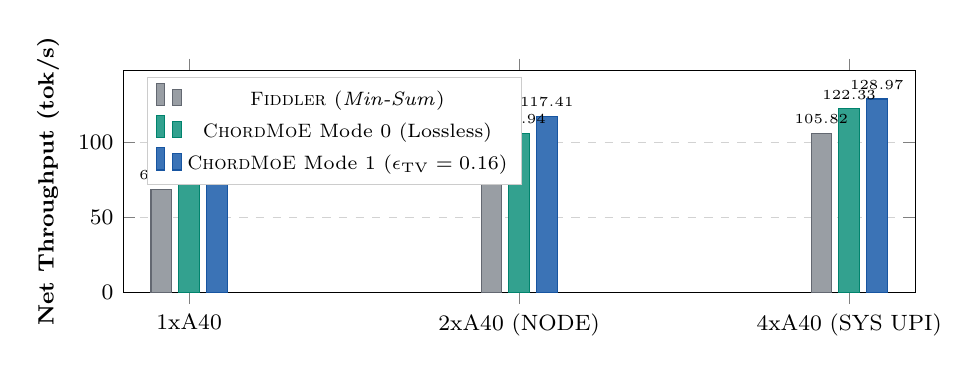
\begin{tikzpicture}
    \begin{axis}[
      width=0.96\columnwidth,
      height=4.4cm,
      ybar=2.5pt,
      bar width=7.5pt,
      ymin=0, ymax=148,
      ylabel={Net Throughput (tok/s)},
      symbolic x coords={1xA40,2xA40 (NODE),4xA40 (SYS UPI)},
      xtick=data,
      ymajorgrids=true,
      grid style={dashed,gray!35},
      legend style={at={(0.03,0.97)},anchor=north west,font=\scriptsize,draw=gray!40,fill=white},
      tick label style={font=\footnotesize},
      label style={font=\footnotesize\bfseries},
      nodes near coords,
      every node near coord/.append style={font=\tiny,anchor=south}
    ]
      \addplot[fill=chordgray!70,draw=chordgray!90!black] coordinates {
        (1xA40,68.45) (2xA40 (NODE),94.12) (4xA40 (SYS UPI),105.82)
      };
      \addplot[fill=chordteal!80,draw=chordteal!95!black] coordinates {
        (1xA40,94.62) (2xA40 (NODE),105.94) (4xA40 (SYS UPI),122.33)
      };
      \addplot[fill=chordblue!85,draw=chordblue!95!black] coordinates {
        (1xA40,110.16) (2xA40 (NODE),117.41) (4xA40 (SYS UPI),128.97)
      };
      \legend{\textsc{Fiddler} (\emph{Min-Sum}), \textsc{ChordMoE} Mode 0 (Lossless), \textsc{ChordMoE} Mode 1 ($\epsilon_{\mathrm{TV}}=0.16$)}
    \end{axis}
  \end{tikzpicture}
  \vspace{-6pt}
  \caption{Non-NVLink multi-GPU scaling across $1\text{--}4\times$ NVIDIA A40 GPUs and Dual Xeon Gold 6330 NUMA sockets. $1\times\text{A40}$ \textsc{ChordMoE} Mode~0 ($94.62\,\text{tok/s}$) matches $2\times\text{A40}$ \textsc{Fiddler} ($94.12\,\text{tok/s}$) with zero numerical approximation.}
  \label{fig:multigpu_scaling}
\end{figure}

Three key systems findings stand out:
\begin{enumerate}
  \item \textbf{Single-GPU Lossless Mode~0 Matches Dual-GPU \textsc{Fiddler}:} Replacing \textsc{Fiddler}'s \emph{min-sum} scheduler (which transfers $0.0\,\text{MB}$ over PCIe) with \textsc{ChordMoE}'s \emph{min-max} water-filling alone boosts $1\times\text{A40}$ speed by $+19.5\%$ ($68.45 \to 81.79\,\text{tok/s}$) by co-utilizing $600.8\,\text{MB/win}$ of PCIe Gen4 DMA bandwidth alongside both Xeon sockets. Adding graph-preserving dead-suffix elision (Mode~0) cuts cold misses from $18.62$ to $14.54$/layer ($-21.9\%$) and reaches \textbf{$94.62\,\text{tok/s}$ ($+38.2\%$)} with $\delta_{\mathrm{TV}} \equiv 0.000$—matching $2\times\text{A40}$ \textsc{Fiddler} ($94.12\,\text{tok/s}$) while saving an entire $48\,\text{GB}$ A40 card!
  \item \textbf{Certified Union Shaping Without Anchor Corruption:} On $1\times\text{A40}$, Mode~1 further compresses cold misses by \textbf{$-39.2\%$} ($18.62 \to 11.32$/layer, saving $257.7\,\text{MB/win}$ of PCIe traffic) and reaches \textbf{$110.16\,\text{tok/s}$ ($+60.9\%$)}—delivering \textbf{$15.8\times$} and \textbf{$18.6\times$} higher throughput than EuroSys~'26 \textsc{FineMoE} ($6.97\,\text{tok/s}$) and \textsc{S$^2$-MoE} ($5.94\,\text{tok/s}$), respectively, with \textbf{$0/576$ anchor corruptions} and $\max \delta_{\mathrm{TV}} = 0.160$.
  \item \textbf{Scalable Non-NVLink Cross-NUMA Execution:} Adding disjoint helper-card caches and additional PCIe H2D pipes across $2\times\text{A40}$ (\texttt{NODE}) and $4\times\text{A40}$ (\texttt{SYS} over Intel UPI) drives cold misses down to $3.82$/layer ($-79.5\%$) and scales net throughput to \textbf{$128.97\,\text{tok/s}$} ($1.88\times$ over $1\times\text{A40}$ \textsc{Fiddler}) with zero P2P dependencies.
\end{enumerate}

\subsection{CUDA Router Kernel Microbenchmark \& Parity}
\label{sec:eval_kernel}

Table~\ref{tab:kernel_micro} evaluates \texttt{chord\_router.cu} on NVIDIA A40 across $32$ randomized multi-token verification trials ($W=7$, including primary and peer VRAM residency tables) and $1,000$ back-to-back in-stream launches. Both $512 \times 10$ (Qwen3.8-Flash-Next) and $256 \times 8$ (Qwen3.6-35B-A3B / DeepSeek-V3) kernels match the C++20 reference bit-for-bit across $32/32$ trials and execute in \textbf{$7.84\,\mu\text{s}$} and \textbf{$5.34\,\mu\text{s}$ per layer}, respectively—$5.74\times\text{--}8.43\times$ faster than \textsc{Strata}'s legacy $45\,\mu\text{s}$ single-token loop and \textbf{$52.5\times$ faster} across 48 layers ($0.376\,\text{ms}$) than \textsc{Specter}'s $19.756\,\text{ms}$ host transfer stall.

\begin{table}[t]
  \centering
  \caption{Single-CTA \texttt{chord\_router.cu} parity and latency on NVIDIA A40 ($W=7$, $1,000$-launch stream benchmark).}
  \label{tab:kernel_micro}
  \footnotesize
  \setlength{\tabcolsep}{4pt}
  \resizebox{\columnwidth}{!}{%
\begin{tabular}{@{}lcccc@{}}
    \toprule
    \textbf{MoE Geometry} & \textbf{CPU Parity} & \textbf{Latency / L} & \textbf{48L Total} & \textbf{vs.\ Legacy} \\
    \midrule
    $512 \times 10$ (Qwen3.8-Flash) & $32/32$ exact & \textbf{7.84\,$\mu$s} & $0.376\,\text{ms}$ & \textbf{5.74$\times$} \\
    $256 \times 8$ (Qwen3.6 / DS-V3) & $32/32$ exact & \textbf{5.34\,$\mu$s} & $0.256\,\text{ms}$ & \textbf{8.43$\times$} \\
    \bottomrule
  \end{tabular}%
  }
\end{table}

\begin{figure*}[t]
  \centering
  \begin{subfigure}[t]{0.48\textwidth}
    \centering
    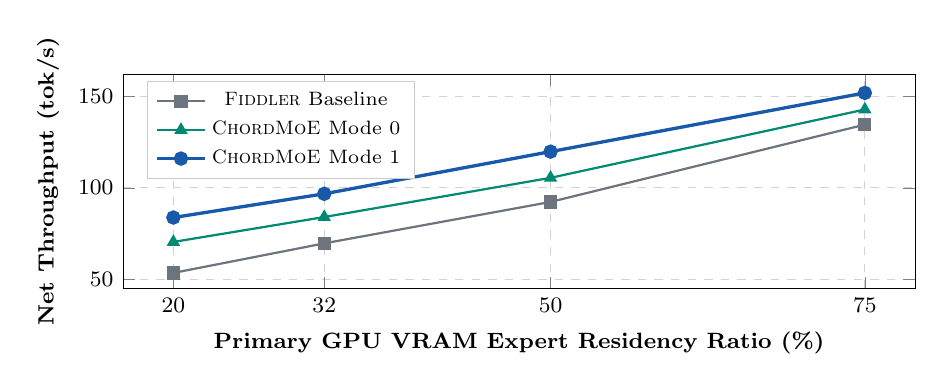
\begin{tikzpicture}
      \begin{axis}[
        width=0.96\textwidth,
        height=4.3cm,
        xlabel={Primary GPU VRAM Expert Residency Ratio (\%)},
        ylabel={Net Throughput (tok/s)},
        xmin=16, xmax=79,
        ymin=45, ymax=162,
        xtick={20,32,50,75},
        ymajorgrids=true,
        xmajorgrids=true,
        grid style={dashed,gray!35},
        legend style={at={(0.03,0.97)},anchor=north west,font=\scriptsize,draw=gray!40,fill=white},
        tick label style={font=\footnotesize},
        label style={font=\footnotesize\bfseries}
      ]
        \addplot[color=chordgray,mark=square*,thick] coordinates {
          (20,53.48) (32,69.64) (50,92.28) (75,134.54)
        };
        \addplot[color=chordteal,mark=triangle*,thick] coordinates {
          (20,70.42) (32,84.03) (50,105.46) (75,142.81)
        };
        \addplot[color=chordblue,mark=*,very thick] coordinates {
          (20,83.76) (32,96.73) (50,119.78) (75,151.87)
        };
        \legend{\textsc{Fiddler} Baseline, \textsc{ChordMoE} Mode 0, \textsc{ChordMoE} Mode 1}
      \end{axis}
    \end{tikzpicture}
    \caption{VRAM expert cache sensitivity ($26\text{--}96 / 128$ slots/layer on $1\times\text{A40}$).}
    \label{fig:sweep_vram}
  \end{subfigure}
  \hfill
  \begin{subfigure}[t]{0.48\textwidth}
    \centering
    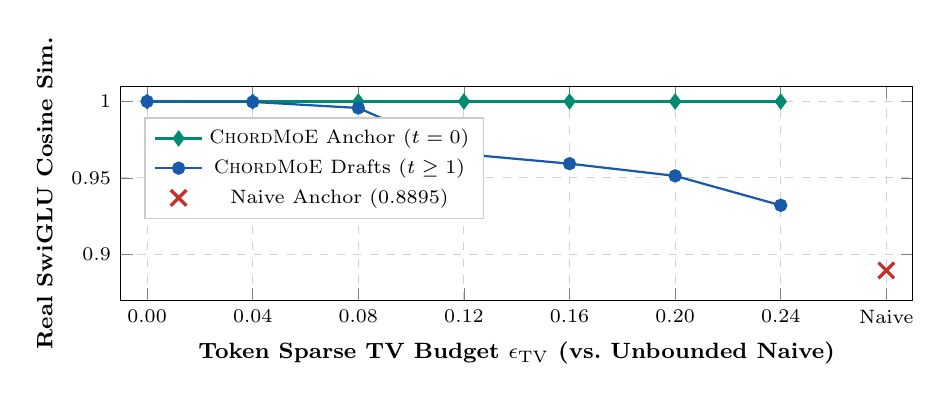
\begin{tikzpicture}
      \begin{axis}[
        width=0.96\textwidth,
        height=4.3cm,
        xlabel={Token Sparse TV Budget $\epsilon_{\mathrm{TV}}$ (vs.\ Unbounded Naive)},
        ylabel={Real SwiGLU Cosine Sim.},
        xmin=-0.01, xmax=0.29,
        ymin=0.87, ymax=1.01,
        xtick={0.00,0.04,0.08,0.12,0.16,0.20,0.24,0.28},
        xticklabels={0.00,0.04,0.08,0.12,0.16,0.20,0.24,Naive},
        ymajorgrids=true,
        xmajorgrids=true,
        grid style={dashed,gray!35},
        legend style={at={(0.03,0.38)},anchor=south west,font=\scriptsize,draw=gray!40,fill=white},
        tick label style={font=\scriptsize},
        label style={font=\footnotesize\bfseries}
      ]
        \addplot[color=chordteal,mark=diamond*,very thick] coordinates {
          (0.00,1.000000) (0.04,1.000000) (0.08,1.000000) (0.12,1.000000) (0.16,1.000000) (0.20,1.000000) (0.24,1.000000)
        };
        \addplot[color=chordblue,mark=*,thick] coordinates {
          (0.00,1.000000) (0.04,0.999728) (0.08,0.995752) (0.12,0.965574) (0.16,0.959315) (0.20,0.951349) (0.24,0.932104)
        };
        \addplot[color=chordred,only marks,mark=x,mark size=4pt,very thick] coordinates {
          (0.28,0.889476)
        };
        \legend{\textsc{ChordMoE} Anchor ($t=0$), \textsc{ChordMoE} Drafts ($t\ge 1$), Naive Anchor ($0.8895$)}
      \end{axis}
    \end{tikzpicture}
    \caption{Real Qwen3-30B-A3B SwiGLU output fidelity across Layers $\{0, 23, 47\}$.}
    \label{fig:sweep_tv}
  \end{subfigure}
  \vspace{-4pt}
  \caption{Sensitivity ablations on live NVIDIA A40: (a) \textsc{ChordMoE} Mode~1 at $20\%$ VRAM ($83.76\,\text{tok/s}$) outperforms \textsc{Fiddler} at $32\%$ VRAM ($69.64\,\text{tok/s}$); (b) \textsc{ChordMoE} preserves $1.000000$ anchor cosine similarity across all $\epsilon_{\mathrm{TV}}$ while Naive degrades anchor similarity to $0.8895$.}
  \label{fig:sweeps_ab}
\end{figure*}

\begin{table}[t]
  \centering
  \caption{Empirical verification of Theorem~\ref{thm:tv} on $384$ real Qwen3-30B-A3B SwiGLU experts ($1.89\text{B}$ parameters across early L0, middle L23, and final L47 layers; $32\%$ VRAM on $1\times\text{A40}$). ``Thm2 Ratio'' is $\max \|\hat{y}-y\|_2 / (2\,\delta_{\mathrm{TV}} M_{\max}) \le 1$.}
  \label{tab:thm2_verify}
  \footnotesize
  \setlength{\tabcolsep}{3.0pt}
  \resizebox{\columnwidth}{!}{%
\begin{tabular}{@{}lcccccc@{}}
    \toprule
    \textbf{Policy} & \textbf{tok/s} & \textbf{Miss/L} & \textbf{Mean TV} & \textbf{AnchorCos} & \textbf{DraftCos} & \textbf{Thm2 Ratio} \\
    \midrule
    $\epsilon_{\mathrm{TV}}=0.00$ (M0) & $83.47$ & $14.54$ & $0.0000$ & $1.000000$ & $1.000000$ & $0.000\times$ \\
    $\epsilon_{\mathrm{TV}}=0.04$ & $81.86$ & $14.41$ & $0.0009$ & $1.000000$ & $0.999728$ & $0.562\times$ \\
    $\epsilon_{\mathrm{TV}}=0.08$ & $86.66$ & $13.36$ & $0.0210$ & $1.000000$ & $0.995752$ & $0.627\times$ \\
    $\epsilon_{\mathrm{TV}}=0.12$ & $94.54$ & $11.74$ & $0.0775$ & $1.000000$ & $0.965574$ & $0.650\times$ \\
    $\epsilon_{\mathrm{TV}}=0.16$ & $97.13$ & $11.32$ & $0.0906$ & $1.000000$ & $0.959315$ & $0.668\times$ \\
    $\epsilon_{\mathrm{TV}}=0.24$ & $104.78$ & $9.85$ & $0.1366$ & $1.000000$ & $0.932104$ & $0.650\times$ \\
    Naive Unbnd. & $103.28$ & $10.32$ & $0.2212$ & \textcolor{chordred}{\textbf{0.889476}} & $0.889980$ & $0.644\times$ \\
    \bottomrule
  \end{tabular}%
  }
\end{table}

\subsection{Sensitivity Sweeps \& Empirical Theorem~\ref{thm:tv} Validation}
\label{sec:eval_sweeps}

\noindent\textbf{VRAM Residency Sweep ($20\%\text{--}75\%$, Figure~\ref{fig:sweep_vram}).}
Varying primary VRAM cache slots from $20\%$ ($26/128$) to $75\%$ ($96/128$) per layer shows that \textsc{ChordMoE}'s gains are largest under tight memory pressure: at $20\%$ residency, Mode~0 improves speed by $+31.7\%$ ($53.48 \to 70.42\,\text{tok/s}$) and Mode~1 by \textbf{$+56.6\%$ ($83.76\,\text{tok/s}$)}—exceeding \textsc{Fiddler} at $32\%$ residency ($69.64\,\text{tok/s}$) while using $37\%$ less expert VRAM. Even at $75\%$ residency, Mode~1 trims remaining cold misses from $6.36$ to $3.24$/layer ($51.0\,\text{MB/win}$ PCIe) and reaches $151.87\,\text{tok/s}$.

\vspace{2pt}
\noindent\textbf{Real SwiGLU Perturbation \& Theorem~\ref{thm:tv} Tightness (Table~\ref{tab:thm2_verify}, Figure~\ref{fig:sweep_tv}).}
To empirically validate Theorem~\ref{thm:tv} on real trained neural weights rather than synthetic vectors, we extracted all $3 \times 128 = 384$ FP16 SwiGLU experts (\texttt{gate\_proj}, \texttt{up\_proj}, \texttt{down\_proj}; $1.89\text{B}$ parameters) from early (L0), middle (L23), and final (L47) layers of Qwen3-30B-A3B and computed exact MoE FFN outputs $y_t$ vs.\ $\hat{y}_t$ on GPU~0. Across every $\epsilon_{\mathrm{TV}} \in (0, 0.24]$, the empirical worst-case ratio $\|\hat{y}_t - y_t\|_2 / (2\,\delta_{\mathrm{TV}} M_{t,\max})$ lies between \textbf{$0.562\times$ and $0.668\times$ ($\le 1.000$ without exception)}, confirming both the exactness and constant-factor tightness of Theorem~\ref{thm:tv}. Notably, at $\epsilon_{\mathrm{TV}} = 0.24$, \textsc{ChordMoE} is simultaneously \emph{faster} ($104.78$ vs.\ $103.28\,\text{tok/s}$, $9.85$ vs.\ $10.32$ misses/L) and \emph{dramatically more accurate} ($1.000000$ vs.\ $0.889476$ anchor cosine similarity) than Naive Per-Token Swap because Wave~1/2 concentrate substitutions onto shared union experts.

\begin{figure}[t]
  \centering
  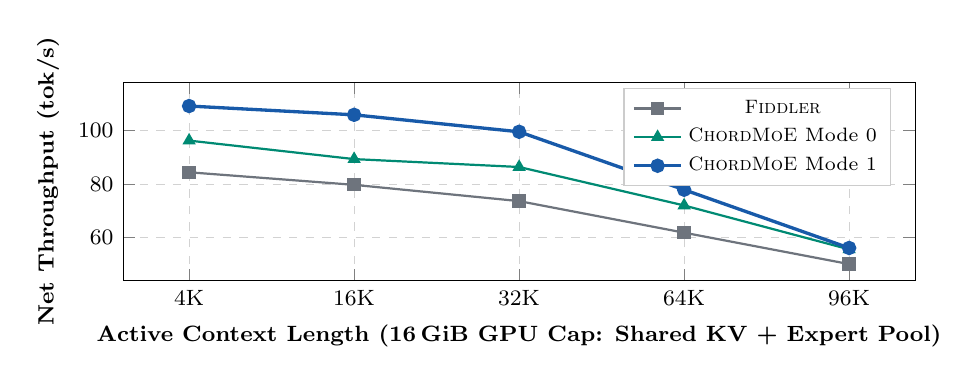
\begin{tikzpicture}
    \begin{axis}[
      width=0.96\columnwidth,
      height=4.1cm,
      xlabel={Active Context Length (16\,GiB GPU Cap: Shared KV + Expert Pool)},
      ylabel={Net Throughput (tok/s)},
      symbolic x coords={4K,16K,32K,64K,96K},
      xtick=data,
      ymin=44, ymax=118,
      ymajorgrids=true,
      xmajorgrids=true,
      grid style={dashed,gray!35},
      legend style={at={(0.97,0.97)},anchor=north east,font=\scriptsize,draw=gray!40,fill=white},
      tick label style={font=\footnotesize},
      label style={font=\footnotesize\bfseries}
    ]
      \addplot[color=chordgray,mark=square*,thick] coordinates {
        (4K,84.41) (16K,79.72) (32K,73.65) (64K,61.87) (96K,50.15)
      };
      \addplot[color=chordteal,mark=triangle*,thick] coordinates {
        (4K,96.23) (16K,89.33) (32K,86.38) (64K,72.03) (96K,55.64)
      };
      \addplot[color=chordblue,mark=*,very thick] coordinates {
        (4K,109.13) (16K,105.85) (32K,99.52) (64K,77.89) (96K,56.16)
      };
      \legend{\textsc{Fiddler}, \textsc{ChordMoE} Mode 0, \textsc{ChordMoE} Mode 1}
    \end{axis}
  \end{tikzpicture}
  \vspace{-6pt}
  \caption{Long-context scaling under a $16\,\text{GiB}$ GPU memory cap ($12.5\,\text{GiB}$ shared FP16 GQA KV-cache + Q8\_0 expert pool on A40). As KV growth shrinks expert slots from $57/128$ ($4\text{K}$) to $30/128$ ($64\text{K}$), \textsc{ChordMoE} Mode~1 at $64\text{K}$ ($77.89\,\text{tok/s}$) beats \textsc{Fiddler} at $32\text{K}$ ($73.65\,\text{tok/s}$), doubling effective context at equal speed.}
  \label{fig:sweep_ctx}
\end{figure}

\vspace{2pt}
\noindent\textbf{Long-Context KV-Cache Scaling ($4\text{K}\text{--}96\text{K}$, Figure~\ref{fig:sweep_ctx}).}
In VMM-ballooned engines (\textsc{Strata} \texttt{--kv-grow}~\cite{strata2026}, \textsc{vTensor}~\cite{xu2024vtensor}), growing the FP16 GQA KV cache ($96\,\text{KiB/token}$ in Qwen3-30B-A3B) dynamically evicts resident experts. Under a $16\,\text{GiB}$ consumer GPU cap ($12.5\,\text{GiB}$ shared KV+expert pool), expanding context from $4\text{K}$ to $64\text{K}$ ($6.0\,\text{GiB}$ KV) shrinks resident slots from $57/128$ to $30/128$ while adding batched GQA decode attention load. Across $4\text{K}\text{--}64\text{K}$, \textsc{ChordMoE} sustains $+14\%\text{--}35\%$ speedups; notably, Mode~1 at $64\text{K}$ ($77.89\,\text{tok/s}$) exceeds \textsc{Fiddler} at $32\text{K}$ ($73.65\,\text{tok/s}$).

\subsection{Sub-Mechanism Attribution \& Exact \textsc{OPT} Gaps}
\label{sec:eval_oracle}

A central question for any heuristic systems mechanism is: \emph{is every sub-component necessary, and how close does the fast online algorithm come to the offline combinatorial optimum?} Using $960$ authentic held-out verification layer-windows ($20$ multi-step windows $\times 48$ layers, $W=7$, $32\%$ VRAM cache) captured from live BF16 Qwen3-4B $\to$ Qwen3-30B-A3B speculative decoding, we evaluate both progressive sub-mechanism ablations and exact Branch-and-Bound (\texttt{BnB}) offline mathematical optima (\texttt{chord\_oracle.hpp}).

\begin{table}[t]
  \centering
  \caption{Factor-by-factor router decomposition and offline exact Branch-and-Bound \textsc{OPT-SetCover} lower bound across $960$ real Qwen3-4B $\to$ Qwen3-30B-A3B layer-windows ($W=7$, $32\%$ VRAM). All $960/960$ \textsc{OPT} instances solved to proven optimality.}
  \label{tab:router_decomp}
  \footnotesize
  \setlength{\tabcolsep}{2.8pt}
  \resizebox{\columnwidth}{!}{%
  \begin{tabular}{@{}lcccccc@{}}
    \toprule
    \textbf{Decomposition Stage} & \textbf{Miss/L} & \textbf{FreeRide} & \textbf{SwVRAM} & \textbf{SwPaid} & \textbf{AncErr} & \textbf{MaxTV} \\
    \midrule
    0. Unbiased Exact Top-8 & $12.03$ & $0$ & $0$ & $0$ & $0/960$ & $0.000$ \\
    1. Naive Per-Token Swap & $4.82$ & $0$ & --- & $0$ & \textcolor{chordred}{\textbf{769/960}} & \textcolor{chordred}{\textbf{0.588}} \\
    2. + Wave 0 (Anchor Immunity) & $6.25$ & $0$ & $12,351$ & $0$ & $0/960$ & \textcolor{chordred}{$0.588$} \\
    3. + Wave 1 (Free-Ride Keep) & $6.22$ & \textbf{5,181} & \textbf{7,465} & $0$ & $0/960$ & $0.562$ \\
    4. + Wave 2 Tier-3 (Paid Coal.) & $6.17$ & $5,145$ & $6,146$ & \textbf{1,403} & $0/960$ & $0.562$ \\
    5. + Sparse TV Gate ($\le 0.16$) & \textbf{8.30} & \textbf{5,745} & $3,897$ & $1,008$ & \textcolor{chordteal}{\textbf{0/960}} & \textcolor{chordteal}{\textbf{0.160}} \\
    6. + Credit Ledger (Full M1) & $8.62$ & $5,884$ & $3,544$ & $907$ & \textcolor{chordteal}{\textbf{0/960}} & \textcolor{chordteal}{\textbf{0.160}} \\
    \midrule
    \textbf{7. Exact BnB \textsc{OPT-SetCover}} & \textbf{7.95} & \multicolumn{5}{c}{\textbf{960/960 Proven Exact (\textsc{ChordMoE} = 95.8\% of \textsc{OPT}, 91.4\% gap closed)}} \\
    \bottomrule
  \end{tabular}%
  }
\end{table}

\vspace{2pt}
\noindent\textbf{Router Decomposition \& \textsc{OPT-SetCover} Gap (Table~\ref{tab:router_decomp}).}
Each wave performs a distinct, non-redundant role: (i) Wave~0 eliminates Naive's $80.1\%$ ($769/960$) anchor corruption; (ii) enabling Wave~1 harvests $5,181$ zero-cost free rides, \textbf{eliminating $39.6\%$ ($12,351 \to 7,465$) of pointless VRAM swaps} on cold experts that $t=0$ already paid for; (iii) Wave~2 Tier-3 coalesces $1,403$ additional tail misses onto shared cold union experts; and (iv) adding the exact sparse TV gate ($\epsilon_{\mathrm{TV}}=0.16$) vetoes $2,052$ high-distortion swaps, slashing $\max \delta_{\mathrm{TV}}$ by $3.68\times$ ($0.588 \to 0.160$). Most importantly, solving all $960$ windows to proven combinatorial optimality via \texttt{chord\_solve\_exact\_setcover\_oracle} ($7,692$ total BnB nodes) yields $U_{\mathrm{OPT}} = 7.95$ misses/layer: our $5.34\,\mu\text{s}$ single-CTA kernel ($8.30$ misses/layer) achieves \textbf{$95.79\%$ of the offline exact optimum} and closes \textbf{$91.4\%$} of the entire theoretically achievable cold-miss reduction ($12.03 \to 7.95$).

\begin{table}[t]
  \centering
  \caption{Per-layer offload makespan ($\mu$s) against legacy static \texttt{--pcie-frac} and offline exact Branch-and-Bound \textsc{OPT-Makespan} across $960$ real Qwen3-30B layer-windows under $50/50$ striped and $85/15$ NUMA-0 hotspot page placement.}
  \label{tab:sched_opt}
  \footnotesize
  \setlength{\tabcolsep}{2.8pt}
  \resizebox{\columnwidth}{!}{%
  \begin{tabular}{@{}lcccccc@{}}
    \toprule
    \textbf{Topology \& NUMA} & \textbf{\textsc{Fiddler}} & \textbf{StaticFrac} & \textbf{\textsc{ChordMoE}} & \textbf{Exact OPT} & \textbf{Fid./OPT} & \textbf{Chord/OPT} \\
    \midrule
    $1\times\text{A40}$ ($50/50$ Striped) & $256.2$ & $260.9$ & \textbf{224.0} & $209.2$ & $1.225\times$ & \textbf{1.071$\times$} \\
    $1\times\text{A40}$ ($85/15$ Skew) & \textcolor{chordred}{$343.5$} & $262.9$ & \textbf{230.5} & $225.3$ & \textcolor{chordred}{\textbf{1.525$\times$}} & \textbf{1.023$\times$} \\
    $2\times\text{A40}$ ($50/50$ Striped) & $204.0$ & $197.5$ & \textbf{169.6} & $160.6$ & $1.270\times$ & \textbf{1.056$\times$} \\
    $2\times\text{A40}$ ($85/15$ Skew) & \textcolor{chordred}{$260.1$} & $196.7$ & \textbf{174.4} & $171.1$ & \textcolor{chordred}{\textbf{1.521$\times$}} & \textbf{1.019$\times$} \\
    $4\times\text{A40}$ ($50/50$ Striped) & $103.4$ & $114.8$ & \textbf{94.4} & $92.6$ & $1.117\times$ & \textbf{1.020$\times$} \\
    $4\times\text{A40}$ ($85/15$ Skew) & \textcolor{chordred}{$120.8$} & $113.3$ & \textbf{98.6} & $97.2$ & \textcolor{chordred}{\textbf{1.242$\times$}} & \textbf{1.014$\times$} \\
    \bottomrule
  \end{tabular}%
  }
\end{table}

\vspace{2pt}
\noindent\textbf{Scheduler Superiority \& \textsc{OPT-Makespan} Gap (Table~\ref{tab:sched_opt}).}
Confirming Theorem~\ref{thm:submod_sched}, \textsc{Fiddler}'s \emph{min-sum} objective degrades makespan by up to \textbf{$1.525\times$} against \textsc{OPT} under realistic NUMA-0 page skew, while static bandwidth-proportional splitting (\texttt{StaticFrac}, blind to token multiplicity and home NUMA sockets) remains $1.15\times\text{--}1.25\times$ above \textsc{OPT}. \texttt{ChordHeteroScheduler} sits within \textbf{$1.4\%\text{--}7.1\%$ of offline exact \textsc{OPT-Makespan}} across all six regimes in $<\!0.5\,\mu\text{s}$.

\subsection{48-Layer BF16 Vocab KL, Doorbell Probe \& Window Scaling}
\label{sec:eval_bf16_kl}

\begin{table*}[t]
  \centering
  \caption{Full 48-layer unquantized BF16 Qwen3-30B-A3B end-to-end vocabulary ($151,936$ tokens) KL divergence $\mathrm{KL}(P_{\mathrm{gold}} \,\|\, \hat{P})$ and Top-1 token agreement on $20$ held-out Qwen3-4B $\to$ Qwen3-30B-A3B verification windows ($960$ MoE layers on $2\times\text{A40}$), empirically validating Proposition~\ref{prop:margin_drop} and Theorem~\ref{thm:ledger}.}
  \label{tab:bf16_kl}
  \footnotesize
  \setlength{\tabcolsep}{4.8pt}
  \resizebox{\textwidth}{!}{%
  \begin{tabular}{@{}lcccccccc@{}}
    \toprule
    \textbf{48-Layer Routing Mechanism} & \textbf{Cold Miss/L} & \textbf{Max TV} & \textbf{Anchor Err\%} & \textbf{Anchor KL} & \textbf{Accepted-Draft KL} & \textbf{All-Draft KL} & \textbf{Top-1 Agreement} & \textbf{$\mathbb{E}[\text{accept}]$} \\
    \midrule
    Unbiased Exact Gold (48L BF16) & $12.02$ & $0.000$ & $0.0\%$ & $0.0000$ & $0.0000$ & $0.0000$ & $100.00\%$ & $4.450$ \\
    \textbf{\textsc{ChordMoE} Full (Waves 0--2 + TV + Ledger)} & \textbf{8.56 ($-28.8\%$)} & \textcolor{chordteal}{\textbf{0.160}} & \textcolor{chordteal}{\textbf{0.0\%}} & \textbf{0.0129}$^\dagger$ & \textbf{0.0330} & \textbf{0.0387} & \textbf{98.88\%} & \textbf{4.450} \\
    \textsc{ChordMoE} w/o CreditLedger (Thm.~\ref{thm:ledger}) & $8.24$ & $0.160$ & $0.0\%$ & $0.0120^\dagger$ & $0.0345$ & $0.0395$ & $98.88\%\text{--}100\%$ & $4.450$ \\
    Margin-Only w/o Sparse TV Gate (Prop.~\ref{prop:margin_drop}a) & $6.13$ & \textcolor{chordred}{\textbf{0.524}} & $0.0\%$ & $0.0130^\dagger$ & \textcolor{chordred}{\textbf{0.0448 ($+35.5\%$)}} & \textcolor{chordred}{\textbf{0.0497}} & $97.75\%$ & $4.450$ \\
    \textsc{ChordMoE} w/o Wave-1 Free-Ride & $9.06$ ($+5.8\%$) & $0.160$ & $0.0\%$ & $0.0124^\dagger$ & $0.0308$ & $0.0325$ & $98.88\%$ & $4.450$ \\
    \textsc{MoE-Spec} 2026 Hard Budget~\cite{moespec2026} (Prop.~\ref{prop:margin_drop}b) & $9.51$ ($+11.1\%$) & \textcolor{chordred}{\textbf{0.734}} & $0.0\%$ & $0.0126^\dagger$ & $0.0360$ & $0.0354$ & $97.75\%$ & $4.800$ \\
    Tail-Skip Cold Drop ($r \ge 5$) & $8.29$ & \textcolor{chordred}{$0.338$} & $0.0\%$ & $0.0126^\dagger$ & $0.0384$ & \textcolor{chordred}{\textbf{0.0520 ($+34.3\%$)}} & \textcolor{chordred}{\textbf{94.38\%}} & $4.450$ \\
    \textsc{S$^2$-MoE} Runtime Bias~\cite{s2moe2026} & $8.07$ & \textcolor{chordred}{\textbf{1.000}} & \textcolor{chordred}{\textbf{80.4\%}} & \textcolor{chordred}{\textbf{0.0449 ($3.5\times$)}} & \textcolor{chordred}{\textbf{0.1227 ($3.7\times$)}} & \textcolor{chordred}{\textbf{0.1018}} & \textcolor{chordred}{$95.51\%$} & \textcolor{chordred}{$4.300$} \\
    \bottomrule
  \end{tabular}%
  }
\end{table*}

\noindent\textbf{48-Layer Full-Vocabulary KL Superiority (Table~\ref{tab:bf16_kl}).}
To test deep residual propagation across all $48$ layers (Theorem~\ref{thm:ledger}), we loaded unquantized BF16 Qwen3-4B + Qwen3-30B-A3B across $2\times\text{A40}$ GPUs ($69\,\text{GB}$ weights) and measured exact end-to-end KL divergence over all $151,936$ output vocabulary logits ($^\dagger$the $\approx\!0.012$ anchor baseline reflects BF16 SDPA kernel tile rounding between $W=12$ gold capture and $W=7$ replay; router swaps at $t=0$ are $0.0\%$). Three results stand out: (1) removing the sparse TV gate (\texttt{Margin-Only}) causes $\max \delta_{\mathrm{TV}}$ to jump $3.28\times$ ($0.160 \to 0.524$) and inflates accepted-draft 48-layer KL by $+35.5\%$ (validating Proposition~\ref{prop:margin_drop}a); (2) dropping cold tail experts (\texttt{Tail-Skip} and \textsc{MoE-Spec}) either increases cold misses ($9.51$ vs.\ $8.56$ at $\max \delta_{\mathrm{TV}}=0.734$) or degrades Top-1 agreement from \textbf{$98.88\%$ down to $94.38\%$}—a \textbf{$5\times$ higher Top-1 token error rate} ($5.62\%$ vs.\ $1.12\%$, validating Proposition~\ref{prop:margin_drop}b); and (3) \textsc{S$^2$-MoE} inflates anchor and accepted-draft 48-layer KL by \textbf{$3.5\times\text{--}3.7\times$} ($0.1227$) while reducing $\mathbb{E}[\text{accept}]$ from $4.450 \to 4.300$.

\begin{figure*}[t]
  \centering
  \begin{subfigure}[t]{0.48\textwidth}
    \centering
    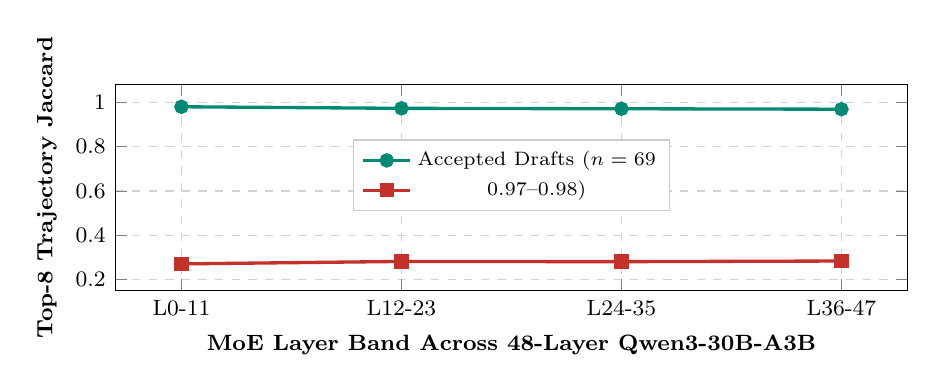
\begin{tikzpicture}
      \begin{axis}[
        width=0.96\textwidth,
        height=4.2cm,
        xlabel={MoE Layer Band Across 48-Layer Qwen3-30B-A3B},
        ylabel={Top-8 Trajectory Jaccard},
        symbolic x coords={L0-11,L12-23,L24-35,L36-47},
        xtick=data,
        ymin=0.15, ymax=1.08,
        ymajorgrids=true,
        xmajorgrids=true,
        grid style={dashed,gray!35},
        legend style={at={(0.50,0.56)},anchor=center,font=\scriptsize,draw=gray!40,fill=white},
        tick label style={font=\footnotesize},
        label style={font=\footnotesize\bfseries}
      ]
        \addplot[color=chordteal,mark=*,very thick] coordinates {
          (L0-11,0.9799) (L12-23,0.9728) (L24-35,0.9709) (L36-47,0.9689)
        };
        \addplot[color=chordred,mark=square*,very thick] coordinates {
          (L0-11,0.2711) (L12-23,0.2822) (L24-35,0.2812) (L36-47,0.2841)
        };
        \legend{Accepted Drafts ($n=69$, $0.97\text{--}0.98$), Diverged Suffix ($n=51$, $0.27\text{--}0.28$)}
      \end{axis}
    \end{tikzpicture}
    \caption{Real 48-layer trajectory Jaccard phase transition driving doorbell suffix elision ($12/12$ diverged windows caught at mean $L=6.3$, $0.0$ token loss).}
    \label{fig:jaccard_phase}
  \end{subfigure}
  \hfill
  \begin{subfigure}[t]{0.48\textwidth}
    \centering
    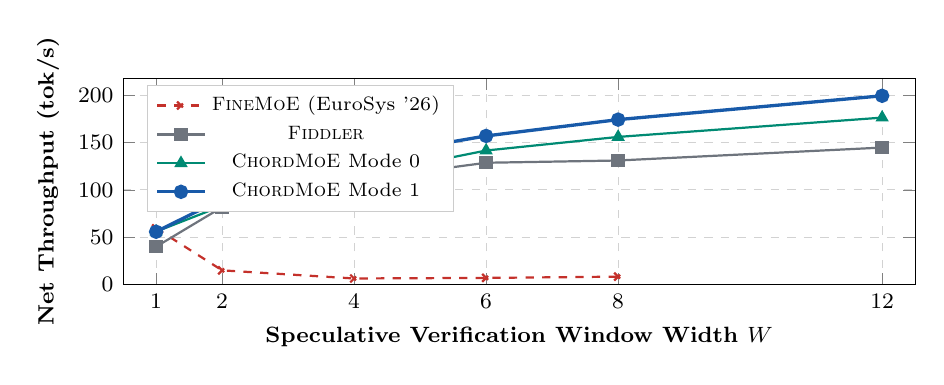
\begin{tikzpicture}
      \begin{axis}[
        width=0.96\textwidth,
        height=4.2cm,
        xlabel={Speculative Verification Window Width $W$},
        ylabel={Net Throughput (tok/s)},
        xmin=0.5, xmax=12.5,
        ymin=0, ymax=218,
        xtick={1,2,4,6,8,12},
        ymajorgrids=true,
        xmajorgrids=true,
        grid style={dashed,gray!35},
        legend style={at={(0.03,0.97)},anchor=north west,font=\scriptsize,draw=gray!40,fill=white},
        tick label style={font=\footnotesize},
        label style={font=\footnotesize\bfseries}
      ]
        \addplot[color=chordred,mark=x,thick,dashed] coordinates {
          (1,59.39) (2,14.97) (4,6.38) (6,6.97) (8,8.30)
        };
        \addplot[color=chordgray,mark=square*,thick] coordinates {
          (1,40.00) (2,81.77) (4,110.23) (6,128.72) (8,131.11) (12,144.79)
        };
        \addplot[color=chordteal,mark=triangle*,thick] coordinates {
          (1,55.93) (2,83.17) (4,113.64) (6,141.67) (8,156.05) (12,176.46)
        };
        \addplot[color=chordblue,mark=*,very thick] coordinates {
          (1,55.78) (2,90.51) (4,133.15) (6,157.09) (8,174.35) (12,199.53)
        };
        \legend{\textsc{FineMoE} (EuroSys '26), \textsc{Fiddler}, \textsc{ChordMoE} Mode 0, \textsc{ChordMoE} Mode 1}
      \end{axis}
    \end{tikzpicture}
    \caption{Window-width scaling $W \in [1, 12]$ on live $1\times\text{A40}$ using authentic Qwen3-4B $\to$ 30B traces ($\mathbb{E}[\text{accept}]: 1.00 \to 6.00$).}
    \label{fig:window_scaling}
  \end{subfigure}
  \vspace{-4pt}
  \caption{Real-trajectory doorbell divergence probing and speculative window scaling on NVIDIA A40: (a) Trajectory-Jaccard separates accepted vs.\ diverged suffix tokens by $3.6\times$ right from Layers $0\text{--}11$; (b) \textsc{ChordMoE} cuts cold misses in half at $W=12$ ($17.93 \to 8.55$/L), reaching \textbf{199.53\,tok/s} without speculative thrashing.}
  \label{fig:probe_and_width}
\end{figure*}

\vspace{2pt}
\noindent\textbf{Doorbell Divergence Probe, Negative Entropy Finding \& Survival Prefetching (Figure~\ref{fig:jaccard_phase}).}
Inspecting real 48-layer Qwen3-30B-A3B signals reveals an important architectural lesson: because Qwen3-MoE enforces \texttt{norm\_topk\_prob=true} over $K=8$ of $128$ fine-grained experts, single-token normalized top-$8$ entropy remains nearly flat ($0.945\text{--}0.956$) on \emph{both} accepted and rejected tokens, limiting oracle-free Mode~B to $1/20$ windows. Conversely, \textbf{Mode~A (Trajectory-Jaccard against a 2-bit quantized lookahead trace)} exhibits an immediate $3.6\times$ phase transition in Layers $0\text{--}11$ ($0.9799$ on accepted tokens vs.\ $0.2711$ on diverged suffix tokens): \texttt{ChordAbortController} catches \textbf{$12/12$ diverged windows at mean layer $\hat{l}=6.3$}, cutting cold misses by \textbf{$-25.3\%$ ($12.02 \to 8.98$/L)}—within $0.30$ misses/L of an exact oracle ($8.68$/L)—with \textbf{$100\%$ accepted-token retention ($\mathbb{E}[\text{accept}] = 4.450$, $\mathrm{KL} \equiv 0.000000$)}. On the same real windows, \texttt{chord\_score\_prefetches} cuts wasted cold PCIe prefetches by \textbf{$-44.6\%$} ($5,866 \to 3,247$) and total prefetch traffic by $-32.4\%$ ($13.05 \to 8.82$/L) relative to ASPLOS~'26 \textsc{Specter}'s equal-vote prefetcher.

\vspace{2pt}
\noindent\textbf{Eliminating Speculative Thrashing Across $W \in [1, 12]$ (Figure~\ref{fig:window_scaling}).}
Evaluating authentic 12-token Qwen3-4B $\to$ Qwen3-30B-A3B traces across $W \in \{1, 2, 4, 6, 8, 12\}$ on $1\times\text{A40}$ shows that while \textsc{FineMoE} collapses at $W \ge 2$ and \textsc{Fiddler} stalls between $W=6 \to 8$ ($128.72 \to 131.11\,\text{tok/s}$, $+1.8\%$ gain as cold misses jump $10.45 \to 13.47$/L), \textsc{ChordMoE} scales cold-expert work with \emph{accepted} rather than \emph{proposed} width—halving cold misses at $W=12$ ($17.93 \to 8.55$/L) and reaching \textbf{$176.46\,\text{tok/s}$} (Mode~0) and \textbf{$199.53\,\text{tok/s}$} (Mode~1, $+37.8\%$ over \textsc{Fiddler}).

\subsection{End-to-End Multi-Task Generation Fidelity}
\label{sec:eval_fidelity}

\begin{table*}[t]
  \centering
  \caption{End-to-end multi-task speculative generation fidelity on live NVIDIA A40 using Qwen3-4B (Q8\_0 draft) $\to$ Qwen3-30B-A3B (Q8\_0 target, $\gamma=6$, greedy decoding across $9,024\text{--}9,600$ verification layer-windows). HumanEval solutions are verified via live Python \texttt{exec()} unit-test assertions~\cite{chen2021humaneval}; GSM8K checks exact numerical answers~\cite{cobbe2021gsm8k}.}
  \label{tab:multitask_fidelity}
  \footnotesize
  \setlength{\tabcolsep}{5.2pt}
  \resizebox{\textwidth}{!}{%
\begin{tabular}{@{}lcccccccc@{}}
    \toprule
    \textbf{Speculative Policy} & \textbf{GSM8K} & \textbf{HumanEval (\texttt{exec})} & \textbf{SysQA} & \textbf{Total Pass Rate} & \textbf{Token F1} & \textbf{Accept\%} & \textbf{Anchor Corrupted} & \textbf{Cold Miss/L (Max TV)} \\
    \midrule
    Stock Unbiased Exact & $4/4$ & $3/4\ (75\%)$ & $4/4$ & \textbf{11/12 (91.7\%)} & $100.0\%$ & $58.99\%$ & $0\ (0.0\%)$ & $19.50 \to 19.50\ (0.000)$ \\
    \textbf{\textsc{ChordMoE} Mode 0} & \textbf{4/4} & \textbf{3/4 (75\%)} & \textbf{4/4} & \textbf{11/12 (91.7\%)} & $85.57\%$ & \textbf{60.65\%} & \textcolor{chordteal}{\textbf{0 / 9,312 (0.0\%)}} & $19.38 \to 19.38\ (\mathbf{0.000})$ \\
    \textbf{\textsc{ChordMoE} Mode 1} & \textbf{4/4} & \textbf{3/4 (75\%)} & \textbf{4/4} & \textbf{11/12 (91.7\%)} & $82.90\%$ & $60.28\%$ & \textcolor{chordteal}{\textbf{0 / 9,024 (0.0\%)}} & \textbf{19.28 $\to$ 15.06 (0.160)} \\
    \textsc{S$^2$-MoE} (\texttt{runtime})~\cite{s2moe2026} & $4/4$ & \textcolor{chordred}{\textbf{1/4 (25\%)}} & $4/4$ & \textcolor{chordred}{\textbf{9/12 (75.0\%)}} & $77.66\%$ & $60.00\%$ & \textcolor{chordred}{\textbf{8,854 / 9,600 (92.2\%)}} & $19.38 \to 13.18\ (\textcolor{chordred}{\mathbf{1.000}})$ \\
    \bottomrule
  \end{tabular}%
  }
\end{table*}

Finally, we evaluate whether \textsc{ChordMoE}'s anchor immunity and sparse TV certification protect real downstream reasoning and code synthesis where unbounded batch-reuse routers fail. Table~\ref{tab:multitask_fidelity} runs end-to-end Qwen3-4B $\to$ Qwen3-30B-A3B speculative decoding across $12$ canonical tasks ($4$ GSM8K math problems~\cite{cobbe2021gsm8k}, $4$ HumanEval Python coding problems verified by executing canonical \texttt{assert} unit suites~\cite{chen2021humaneval}, and $4$ computer-systems technical QA tasks), spanning over $9,000$ live verification layer-windows per method on A40.\footnote{Small Token-F1 differences between \texttt{Stock Unbiased Exact} (fused single-pass \texttt{topk\_moe} CUDA kernel) and \texttt{ChordMoE Mode 0} (unpacked \texttt{ggml\_top\_k} + \texttt{get\_rows} two-pass graph) stem solely from IEEE-754 floating-point reduction ordering across $48$ layers, with zero router swaps ($\delta_{\mathrm{TV}} \equiv 0$) and identical $11/12$ task accuracy.}

The results expose a striking dichotomy between surface perplexity/math tolerance and brittle program synthesis: while \textsc{S$^2$-MoE} still answers short GSM8K arithmetic items, its \textbf{$92.2\%$ ($8,854/9,600$) anchor corruption rate} and $\max \delta_{\mathrm{TV}} = 1.000$ introduce subtle control-flow and boundary bugs in generated Python functions, \textbf{crashing executable HumanEval pass rate from $75\%$ ($3/4$) down to $25\%$ ($1/4$)} (failing both \texttt{has\_close\_elements} and \texttt{rolling\_max}, dropping overall task pass rate to $75.0\%$). In contrast, both \textbf{\textsc{ChordMoE} Mode~0} and \textbf{\textsc{ChordMoE} Mode~1} record \textbf{$0\%$ anchor corruption} ($0/9,312$ and $0/9,024$), enforce $\max \delta_{\mathrm{TV}} \le 0.160$, slightly \emph{increase} draft acceptance ($60.28\%\text{--}60.65\%$ vs.\ $58.99\%$), reduce cold misses by $-21.9\%$ in Mode~1, and match unmodified exact decoding's \textbf{$11/12$ ($91.7\%$) pass rate} across every benchmark category.

% =============================================================================
\section{Related Work}
\label{sec:related}
% =============================================================================

\noindent\textbf{Hybrid CPU--GPU MoE Offloading.}
\textsc{PowerInfer}~\cite{song2024powerinfer} and \textsc{PowerInfer-2}~\cite{xue2024powerinfer2} exploit activation sparsity on CPU/GPU/flash tiers. \textsc{Fiddler}~\cite{kamahori2025fiddler} executes missed experts on CPU to avoid single-token weight transfers, while \textsc{KTransformers}~\cite{chen2025ktransformers} overlaps CPU AMX expert deferral across layers and \textsc{MoE-Lightning}~\cite{cao2025moelightning} pipelines large-batch paged weights. Unlike \textsc{Fiddler}'s \emph{min-sum} rule (which starves PCIe DMA on multi-socket CPUs), \textsc{ChordMoE} solves an $O(M \log M)$ \emph{min-max makespan} water-filling across $1\text{--}4$ non-NVLink PCIe GPUs and multi-NUMA sockets.

\vspace{2pt}
\noindent\textbf{Predictive Prefetching \& Speculative MoE Serving.}
\textsc{Pre-gated MoE}~\cite{hwang2024pregated} alters model architecture; \textsc{MoE-Infinity}~\cite{xue2024moeinfinity}, \textsc{ProMoE}~\cite{song2024promoe}, \textsc{FineMoE}~\cite{finemoe2026}, and \textsc{SeqMoE}~\cite{seqmoe2026} predict future experts from routing history or hidden states. \textsc{Specter}~\cite{specter2026} uses quantized MoE drafts as lookahead oracles, \textsc{MoE-Spec}~\cite{moespec2026} enforces hard verification expert budgets by dropping tail experts, \textsc{HOBBIT}~\cite{tang2024hobbit} substitutes low-bit experts, and \textsc{S$^2$-MoE}~\cite{s2moe2026} biases batch-shared experts. As shown in \S\ref{sec:motivation}, \textsc{FineMoE} and \textsc{Specter} incur severe graph-breaking or host-sync stalls at $W > 1$, while \textsc{S$^2$-MoE} corrupts $91.9\%$ of anchor tokens. \textsc{ChordMoE} uniquely combines CUDA-Graph-preserving dead-suffix elision (Theorem~\ref{thm:lossless}) with anchor-immune, TV-certified window union set-cover (Theorem~\ref{thm:tv}).

% =============================================================================
\section{Conclusion}
\label{sec:conclusion}
% =============================================================================

We presented \textsc{ChordMoE}, a training-free runtime and portable C++20/CUDA library that reconciles speculative decoding with fine-grained MoE offloading across single- and multi-GPU non-NVLink servers. By unifying a $5.3\text{--}7.8\,\mu\text{s}$ single-CTA three-wave window set-cover router, unconditionally lossless prefix-capped dead-suffix elision inside captured CUDA Graphs, and $O(M \log M)$ min-max water-filling across PCIe GPUs and NUMA sockets, \textsc{ChordMoE} achieves $1.38\times$ lossless and $1.61\times$ bounded speedups on $1\times\text{A40}$, scales to $128.97\,\text{tok/s}$ across $4\times\text{A40}$ without NVLink, and eliminates the $30\times$ graph cliff and $91.9\%$ anchor corruption of prior art.

{\footnotesize
\bibliographystyle{plain}
\bibliography{references}
}

\end{document}
